\documentclass[compsoc,conference,letterpaper,fleqn]{IEEEtran}
 
\usepackage{cite}
\usepackage{amsmath,amsfonts,amssymb,amsthm}
\usepackage{thmtools}
\usepackage{stmaryrd}
\usepackage{natbib}
\usepackage{url}
\usepackage{array}
\usepackage{arydshln}
\usepackage{ifthen}
\usepackage{ifpdf}
\usepackage{verbatim}
\usepackage{mathpartir}
\usepackage{listings}
\usepackage{hyperref}
\usepackage{multicol}
\usepackage{natbib}
\lstset{
  basicstyle=\footnotesize\ttfamily,
  columns=fullflexible,
  keepspaces=true,
  mathescape
}

\usepackage{rotating}
\usepackage{afterpage}

\usepackage{mathtools}
\DeclarePairedDelimiter\ceil{\lceil}{\rceil}
\DeclarePairedDelimiter\floor{\lfloor}{\rfloor}

\usepackage{enumitem}
\newlist{enumproof}{enumerate}{10}
\setlist[enumproof]{label*=\arabic*.}

\usepackage{tikz}
\usetikzlibrary{positioning}
\usepackage{multirow,bigdelim}

\ifCLASSOPTIONcompsoc
\usepackage[caption=false,font=normalsize,labelfont=sf,textfont=sf]{subfig}
\else
\usepackage[caption=false,font=footnotesize]{subfig}
\fi



% Include the following to reduce room around display equations
%\setlength{\abovedisplayskip}{3pt}
%\setlength{\belowdisplayskip}{3pt}
%\setlength{\abovedisplayshortskip}{3pt}
%\setlength{\belowdisplayshortskip}{3pt}

% %make latex preview-mode work with natbib...
% \usepackage[displaymath,floats,graphics,textmath,footnotes]{preview}

\newtheorem{theorem}{Theorem}
\newtheorem{lemma}{Lemma}

\newcommand{\forcenewline}{$\phantom{v}$\\}
\newcommand{\judgment}[2]{\paragraph{#1}\hspace{\stretch{1}}\fbox{$#2$}}

\newcommand{\update}[2]{[#1 \mapsto #2]}
\newcommand{\sem}[1]{\left\llbracket #1 \right\rrbracket}

% Math notation
\newcommand{\restrictfun}[1]{|_{#1}}
\newcommand{\parfun}{\rightharpoonup}
\newcommand{\finparfun}{\xrightharpoonup{\textit{\tiny{fin}}}}
\newcommand{\monnefun}{\xrightarrow{\textit{\tiny{mon, ne}}}}
\newcommand{\monfun}{\xrightarrow{\textit{\tiny{mon}}}}
\newcommand{\nefun}{\xrightarrow{\textit{\tiny{ne}}}}
\newcommand{\fun}{\rightarrow}
\newcommand{\defeq}{\stackrel{\textit{\tiny{def}}}{=}}
\newcommand{\nequal}[1][n]{\stackrel{\tiny{#1}}{=}}
\renewcommand{\nsim}[1][n]{\stackrel{\tiny{#1}}{\simeq}}

\newcommand\subsetsim{\mathrel{\ooalign{\raise.2ex\hbox{$\subset$}\cr
      \hidewidth\lower.8ex\hbox{\scalebox{0.9}{$\sim$}}\hidewidth\cr}}}
\newcommand\supsetsim{\mathrel{\ooalign{\raise.2ex\hbox{$\supset$}\cr
      \hidewidth\lower.8ex\hbox{\scalebox{0.9}{$\sim$}}\hidewidth\cr}}}
\newcommand{\nsubsim}[1][n]{\stackrel{\tiny{#1}}{\subsetsim}}
\newcommand{\nsupsim}[1][n]{\stackrel{\tiny{#1}}{\supsetsim}}

\newcommand{\nsubeq}[1][n]{\stackrel{\tiny{#1}}{\subseteq}}
\newcommand{\nsupeq}[1][n]{\stackrel{\tiny{#1}}{\supseteq}}

\newcommand{\union}{\mathbin{\cup}}
\DeclareMathOperator{\dom}{dom}
\newcommand{\blater}{\mathop{\blacktriangleright}}
\newcommand{\id}{\var{id}}
\newcommand{\undefined}{\mathit{undefined}}

\newcommand{\powerset}[1]{\mathcal{P}(#1)}

\newcommand{\false}{\mathit{false}}
\newcommand{\true}{\mathit{true}}


% cofes
\newcommand{\cofe}{c.o.f.e.}
\newcommand{\cofes}{\cofe{}'s}
\newcommand{\CatC}{\mathbb{C}}
\newcommand{\CatP}{\mathbb{P}}

% Comments
\newcommand\lau[1]{{\color{purple} \sf \footnotesize {LS: #1}}\\}
\newcommand\dominique[1]{{\color{purple} \sf \footnotesize {DD: #1}}\\}
\newcommand\lars[1]{{\color{purple} \sf \footnotesize {LB: #1}}\\}

% Variables
\newcommand{\var}[1]{\mathit{#1}}
\newcommand{\hs}{\var{ms}}
\newcommand{\ms}{\hs}
\newcommand{\hv}{\var{r}}
\newcommand{\rv}{\var{r}}
\newcommand{\lv}{\var{r}}
\newcommand{\gl}{\var{g}}
\newcommand{\pc}{\mathit{pc}}
\newcommand{\pcreg}{\mathrm{pc}}
\newcommand{\addr}{\var{a}}
\newcommand{\offset}{\var{offset}}
\newcommand{\word}{\var{w}}
\newcommand{\start}{\var{b}}
\newcommand{\addrend}{\var{e}}
\newcommand{\pwlv}{\var{pwl}}
\newcommand{\mem}{\var{mem}}
\newcommand{\reg}{\var{reg}}
\newcommand{\heapseg}{\var{ms}}
\newcommand{\heap}{\var{mem}}
\newcommand{\mode}{\var{mode}}
\newcommand{\perm}{\var{perm}}
\newcommand{\permp}{\var{permPair}}
\newcommand{\roll}{\var{roll}}
\newcommand{\instr}{\var{instr}}
\newcommand{\stdcap}[1][(\perm,\gl)]{\left(#1,\start,\addrend,\addr \right)}
\newcommand{\adv}{\var{adv}}
\newcommand{\msframe}{ms_\var{frame}}
\newcommand{\link}{\var{link}}
\newcommand{\stk}{\var{stk}}
\newcommand{\flag}{\var{flag}}
\newcommand{\nwl}{\var{nwl}}
\newcommand{\pwl}{\var{pwl}}
\newcommand{\sta}{\var{sta}}
\newcommand{\cnst}{\var{cnst}}
\newcommand{\olf}{\var{offsetLinkFlag}}
\newcommand{\prp}{\var{prp}}
\newcommand{\env}{\var{env}}
\newcommand{\cls}{\var{cls}}
\newcommand{\unused}{\var{unused}}
\newcommand{\act}{\var{act}}


% Memory projections
\newcommand{\plainproj}[1]{\mathrm{#1}}
\newcommand{\memheap}[1][\Phi]{#1.\plainproj{mem}}
\newcommand{\memreg}[1][\Phi]{#1.\plainproj{reg}}

\newcommand{\updateHeap}[3][\Phi]{#1\update{\plainproj{mem}.#2}{#3}}
\newcommand{\updateReg}[3][\Phi]{#1\update{\plainproj{reg}.#2}{#3}}

% Configuration end states
\newcommand{\failed}{\mathit{failed}}
\newcommand{\halted}{\mathit{halted}}

% Functions
\newcommand{\plainfun}[2]{
  \ifthenelse{\equal{#2}{}}
  {\mathit{#1}}
  {\mathit{#1}(#2)}
}
\newcommand{\decode}{\plainfun{decode}{}}
\newcommand{\encode}{\plainfun{encode}{}}
\newcommand{\encodePerm}{\mathit{encodePerm}}
\newcommand{\encodePermPair}{\plainfun{encodePermPair}{}}
\newcommand{\encodeLoc}{\mathit{encodeLoc}{}}
\newcommand{\decodePermPair}{\plainfun{decodePermPair}}
\newcommand{\decodePerm}[1]{\plainfun{decodePerm}{#1}}
\newcommand{\updatePcPerm}[1]{\plainfun{updatePcPerm}{#1}}

\newcommand{\executeAllowed}[1]{\plainfun{executeAllowed}{#1}}
\newcommand{\nonZero}[1]{\plainfun{nonZero}{#1}}
\newcommand{\readAllowed}[1]{\plainfun{readAllowed}{#1}}
\newcommand{\writeAllowed}[1]{\plainfun{writeAllowed}{#1}}
\newcommand{\withinBounds}[1]{\plainfun{withinBounds}{#1}}
\newcommand{\stdUpdatePc}[1]{\plainfun{updatePc}{#1}}

\newcommand{\readCond}[1]{\plainfun{readCondition}{#1}}
\newcommand{\writeCond}[1]{\plainfun{writeCondition}{#1}}
\newcommand{\execCond}[1]{\plainfun{executeCondition}{#1}}
\newcommand{\entryCond}[1]{\plainfun{enterCondition}{#1}}

\newcommand{\revokeTemp}[1]{\plainfun{revokeTemp}{#1}}
\newcommand{\erase}[2]{\floor*{#1}_{\{#2\}}}
\newcommand{\activeReg}[1]{\plainfun{active}{#1}}

% World operations
\newcommand{\future}{\mathbin{\sqsupseteq}}
\newcommand{\pub}{\var{pub}}
\newcommand{\priv}{\var{priv}}
\newcommand{\futurewk}{\mathbin{\sqsupseteq}^{\var{pub}}}
\newcommand{\futurestr}{\mathbin{\sqsupseteq}^{\var{priv}}}
\newcommand{\heapSat}[3][\heap]{#1 :_{#2} #3}
\newcommand{\memSat}[3][n]{\heapSat[#2]{#1}{#3}}
\newcommand{\memSatPar}[4][n]{\heapSat[#2]{#1 , #4}{#3}}

\newcommand{\monwknefun}{\xrightarrow[\text{\tiny{$\futurewk$}}]{\textit{\tiny{mon, ne}}}}
\newcommand{\monstrnefun}{\xrightarrow[\text{\tiny{$\futurestr$}}]{\textit{\tiny{mon, ne}}}}


% Assembly labels
\newcommand{\codelabel}[1]{\mathit{#1}}
\newcommand{\init}{\codelabel{init}}
\newcommand{\malloc}{\codelabel{malloc}}
\newcommand{\counter}{\codelabel{counter}}
\newcommand{\iocap}{\codelabel{iocap}}

% Type(s)
\newcommand{\type}[1]{\mathrm{#1}}
\newcommand{\asmType}{\plaindom{AsmType}}


% Domains
\newcommand{\plaindom}[1]{\mathrm{#1}}
\newcommand{\Caps}{\plaindom{Cap}}
\newcommand{\Words}{\plaindom{Word}}
\newcommand{\Addrs}{\plaindom{Addr}}
\newcommand{\ExecConfs}{\plaindom{ExecConf}}
\newcommand{\RegName}{\plaindom{RegName}}
\newcommand{\Regs}{\plaindom{Reg}}
\newcommand{\Heaps}{\plaindom{Mem}}
\newcommand{\Mems}{\Heaps}
%\newcommand{\HeapSegments}{\plaindom{MemSegment}}
\newcommand{\HeapSegments}{\plaindom{MemSeg}}
\newcommand{\MemSegments}{\HeapSegments}
\newcommand{\Confs}{\plaindom{Conf}}
\newcommand{\Instrs}{\plaindom{Instructions}}
\newcommand{\nats}{\mathbb{N}}
\newcommand{\ints}{\mathbb{Z}}
\newcommand{\Perms}{\plaindom{Perm}}
\newcommand{\Globals}{\plaindom{Global}}

\newcommand{\Rel}{\plaindom{Rel}}
\newcommand{\Rels}{\plaindom{Rels}}
\newcommand{\States}{\plaindom{State}}
\newcommand{\RegionNames}{\plaindom{RegionName}}
\newcommand{\Regions}{\plaindom{Region}}
\newcommand{\Reg}{\plaindom{Reg}}
\newcommand{\Worlds}{\plaindom{World}}
\newcommand{\Wor}{\plaindom{Wor}}
\newcommand{\Worwk}{\Wor_{\futurewk}}
\newcommand{\Worstr}{\Wor_{\futurestr}}
\newcommand{\xiwk}{\xi_{\var{wk}}}
\newcommand{\xistr}{\xi_{\var{str}}}
\newcommand{\StorePred}{\plaindom{MemSegPred}}
\newcommand{\UPred}[1]{\plaindom{UPred}(#1)}
\newcommand{\DCPred}[1]{\plaindom{P}^\downarrow(#1)}

\newcommand{\Views}{\plaindom{View}}

% LR
\newcommand{\intr}[2]{\mathcal{#1}}
\newcommand{\valueintr}[1]{\intr{V}{#1}}
\newcommand{\exprintr}[1]{\intr{E}{#1}}
\newcommand{\contintr}[1]{\intr{K}{#1}}
\newcommand{\regintr}[1]{\intr{R}{#1}}
\newcommand{\stdvr}{\valueintr{\asmType}}
\newcommand{\stder}{\exprintr{\asmType}}
\newcommand{\stdrr}{\regintr{\asmType}}
\newcommand{\stdkr}{\contintr{\asmType}}
\newcommand{\observations}{\mathcal{O}}
\newcommand{\npair}[2][n]{\left(#1,#2 \right)}
\newcommand{\npairP}[2][n]{(#1,#2)}

% Reference register/memory
\newcommand{\refreg}[1]{#1}
\newcommand{\refheap}[1]{#1}

% Instructions
% No arguments
\newcommand{\zinstr}[1]{\mathtt{#1}}
\newcommand{\fail}{\zinstr{fail}}
\newcommand{\halt}{\zinstr{halt}}
% One argument
\newcommand{\oneinstr}[2]{
  \ifthenelse{\equal{#2}{}}
  {\zinstr{#1}}
  {\zinstr{#1} \; #2}
}
\newcommand{\jmp}[1]{\oneinstr{jmp}{#1}}
% Two arguments
\newcommand{\twoinstr}[3]{
  \ifthenelse{\equal{#2#3}{}}
  {\zinstr{#1}}
  {\zinstr{#1} \; #2 \; #3}
}
\newcommand{\restricttwo}[2]{\twoinstr{restrict}{#1}{#2}}
\newcommand{\jnz}[2]{\twoinstr{jnz}{#1}{#2}}
\newcommand{\isptr}[2]{\twoinstr{isptr}{#1}{#2}}
\newcommand{\geta}[2]{\twoinstr{geta}{#1}{#2}}
\newcommand{\getb}[2]{\twoinstr{getb}{#1}{#2}}
\newcommand{\gete}[2]{\twoinstr{gete}{#1}{#2}}
\newcommand{\getp}[2]{\twoinstr{getp}{#1}{#2}}
\newcommand{\getl}[2]{\twoinstr{getl}{#1}{#2}}
\newcommand{\move}[2]{\twoinstr{move}{#1}{#2}}
\newcommand{\store}[2]{\twoinstr{store}{#1}{#2}}
\newcommand{\load}[2]{\twoinstr{load}{#1}{#2}}
\newcommand{\lea}[2]{\twoinstr{lea}{#1}{#2}}
% Three arguments
\newcommand{\threeinstr}[4]{
  \ifthenelse{\equal{#2#3#4}{}}
  {\zinstr{#1}}
  {\zinstr{#1} \; #2 \; #3 \; #4}
}
\newcommand{\restrict}[3]{\threeinstr{restrict}{#1}{#2}{#3}}
\newcommand{\subseg}[3]{\threeinstr{subseg}{#1}{#2}{#3}}
\newcommand{\plus}[3]{\threeinstr{plus}{#1}{#2}{#3}}
\newcommand{\minus}[3]{\threeinstr{minus}{#1}{#2}{#3}}

% Permissions
\newcommand{\plainperm}[1]{\mathrm{#1}}
\newcommand{\noperm}{\plainperm{o}}
\newcommand{\readonly}{\plainperm{ro}}
\newcommand{\readwrite}{\plainperm{rw}}
\newcommand{\exec}{\plainperm{rx}}
\newcommand{\entry}{\plainperm{e}}
\newcommand{\rwx}{\plainperm{rwx}}
% PWL permissions
\newcommand{\readwritel}{\plainperm{rwl}}
\newcommand{\rwl}{\readwritel}
\newcommand{\rwlx}{\plainperm{rwlx}}

% Global/local
\newcommand{\local}{\plainperm{local}}
\newcommand{\glob}{\plainperm{global}}

\newcommand{\localityReg}{\var{localityReg}}
\newcommand{\localReg}{\var{localReg}}
\newcommand{\globalReg}{\var{globalReg}}

% Views
\newcommand{\plainview}[1]{\mathrm{#1}}
\newcommand{\perma}{\plainview{perm}}
\newcommand{\temp}{\plainview{temp}}
\newcommand{\revoked}{\plainview{revoked}}

% OP sem
\newcommand{\diverge}[1][n]{\not\Downarrow_{#1}}
\newcommand{\step}[1][]{\rightarrow_{#1}}

% Conv defs
\newcommand{\lookingat}[3]{\ensuremath{#1} \text{ is looking at } \ensuremath{#2} \text{ followed by } \ensuremath{#3}}
\newcommand{\pointstostack}[3]{\ensuremath{#1} \text{ points to stack with } \ensuremath{#2} \text{ used and } \ensuremath{#3} \text{ unused}}
\newcommand{\nonlocal}[1]{\ensuremath{#1} \text{ is non-local}}

% Macros
\newcommand{\scall}[3]{\mathtt{scall} \; #1([#2],[#3])}


\newcommand{\isdef}{\mathrel{\overset{\makebox[0pt]{\mbox{\normalfont\tiny\sffamily def}}}{=}}}
\newcommand\bnfdef{\mathrel{::=}}

\usepackage[colorinlistoftodos,prependcaption,textsize=tiny]{todonotes}


% domi: IEEEtran.cls sets font size to 10bp, apparently.
% not sure what the difference is with 10pt.
\DeclareMathSizes{10bp}{8}{7}{6}

%\def\IEEEbibitemsep{0pt}

\makeatletter
\setlength\mpr@andskip{1em}
\def\mpr@lineskip{5em}
\def\MathparLineskip{\mpr@lesslineskip}
\makeatother

\newlength{\oldmathindent}
\newenvironment{withmathindent}[1]{\setlength{\oldmathindent}{\mathindent}\setlength{\mathindent}{#1}}{\setlength{\mathindent}{\oldmathindent}}


\begin{document}
\setlength{\mathindent}{.2cm}

\title{Reasoning about a Capability Machine with Local Capabilities\\
 Provably Safe Stack and Return Pointer Management (without OS Support)}


% \author{%
% \IEEEauthorblockN{Lau~Skorstengaard}
% \IEEEauthorblockA{Aarhus University, Denmark\\
% Email: lau@cs.au.dk} \and
% \IEEEauthorblockN{Dominique~Devriese}
%   \IEEEauthorblockA{iMinds-DistriNet, KU Leuven, Belgium\\
% Email: dominique.devriese@cs.kuleuven.be} \and
% \IEEEauthorblockN{Lars~Birkedal}\IEEEauthorblockA{Aarhus University, Denmark\\
% Email: birkedal@cs.au.dk}}
\author{}
\maketitle

\begin{abstract}  
  Capability machines provide security guarantees at machine level which makes
  them an interesting target for compilation schemes that aim to provably
  enforce properties like control-flow correctness, encapsulation of local
  state. We provide a formalisation of a representative capability machine and
  propose a novel calling convention for enforcing control-flow correctness and
  encapsulation of local state on it. To prove these properties, we provide a
  logical relation that semantically captures the guarantees provided by the
  hardware (a form of capability safety). These results are not tied to our
  calling convention and can be used to reason about arbitrary programs.
\end{abstract}

% \section*{Terminology ?}

% \emph{capability safe}: 
% Our unary logical relation is a semantic \emph{definition}
% of which values for the
% pc / register-file / word are capability safe. 

% \emph{adversary}: It doesn't sound ``sexy'' to constantly say ``an untrusted
% piece of code'' should we adopt the convention that adversary refers
% to an unstrusted piece of code?

% \emph{memory}  we don't make a distinction between memory and memory
% segments in the text  (to do so properly, we would need to explain why
% assumptions
% are reasonable, given that a real machine has finite memory, but we
% need infinite domain for malloc spec, etc.)


\section{Introduction}
\label{sec:introduction}

Compromising software security is often based on attacks that break programming
language properties relied upon by software authors, such as control-flow
correctness, local state encapsulation, etc. Commodity processors offer little
support for defending against such attacks: they offer security primitives with
only coarse-grained memory protection and limited compartmentalization
scalability. As a result, defenses against attacks on control-flow correctness
and local state encapsulation are either limited to only certain common forms of
attacks (leading to an attack-defense arms race) or rely on techniques like
machine code rewriting
(e.g.,~\cite{wahbe_efficient_1993,abadi_control-flow_2005}), machine code
verification (e.g.,~\cite{morrisett_system_1999}), virtual machines with a
native stack (e.g.,~the JVM~\citep{lindholm_java_2014}) or
randomization~\citep{forrest_building_1997}. The latter techniques essentially
emulate protection techniques on existing hardware, at the cost of performance,
system complexity and/or security.

\emph{Capability machines} are a type of processors, intended to
remediate these limitations by presenting a better security model at
the hardware level. They are based on old ideas
(e.g.~\cite{Carter:1994:HSF:195473.195579,Dennis:1966:PSM:365230.365252,shapiro_eros:_1999}),
but have recently received renewed interest; in particular, the CHERI
project has proposed new ideas and ways of tackling practical
challenges like backwards compatibility and realistic OS
support~\citep{Watson2015Cheri,Woodruff:2014:CCM:2665671.2665740}. Capability
machines tag every word (in the register file and in memory) to
enforce a strict separation between numbers and capabilities, a kind
of pointers carrying some kind of authority. Memory capabilities carry
the authority to read and/or write to a range of memory
locations. Moreover, all capability machines
offer some form of \emph{object capabilities}, which represent the
authority to invoke a piece of code without exposing the code's
encapsulated private state (e.g., the M-Machine's enter capabilities or
CHERI's sealed code/data pairs).

In contrast to the situation for commodity processors, the security
primitives on capability machines lend themselves well to the
enforcement of properties like local state encapsulation and
control-flow correctness. Potentially, they will enable new compilation
schemes that enforce such properties in a way that is efficient but
also 100\% watertight (ideally evidenced by a mathematical proof,
guaranteeing that we do not end up in a new attack-defense arms
race). However, there is still a lot that needs to happen to attain
this goal. For example, it is quite non-trivial to devise a
compilation scheme adapted to the details of a specific language's
notion of encapsulation (e.g., encapsulation of private member
variables in OO languages often behaves quite differently than
encapsulation of private state in ML-like languages). And even if such
a scheme were defined, a formal proof depends on a formalisation of
the encapsulation provided by the capability machine at hand.

A similar problem is the enforcement of control-flow correctness on capability
machines. An interesting approach is taken in CheriBSD~\citep{Watson2015Cheri}:
It drops the standard contiguous C stack and splits it into a central, trusted
shadow stack, managed by trusted call and return instructions, and disjoint,
per-component stacks. To prevent illegal use of stack references, the approach
relies on \emph{local capabilities}, a type of capabilities offered by CHERI
that can be passed over a function invocation \emph{temporarily}, for the
duration of the invocation, and revoked afterwards. However, a lot of details
remain to be investigated (e.g., how to combine a trusted shadow stack with
(potentially) cross-domain function pointers in a scalable way?) and there is no
argument that this enforcement of control-flow correctness is watertight.

In this paper, we make progress towards the goal of efficient and provably
watertight enforcement of encapsulation and control-flow correctness on
capability machines. Specifically, we make the following contributions:
\begin{itemize}
\item Formalise a simple but representative capability machine featuring local
  capabilities, and its operational semantics
  (Section~\ref{sec:capab-mach-with})
\item Define a novel calling convention enforcing control-flow correctness and
  encapsulation of local state on the stack
  (Section~\ref{sec:stack-and-return-pointer}). It relies solely on local
  capabilities and does not require OS support (like a trusted stack or
  call/return instructions). It also does not use separate per-component stacks
  but a single, fairly standard, contiguous stack. It supports higher-order
  cross-component calls (e.g., (potentially) cross-component function pointers)
  and can be efficient assuming only one additional piece of processor support:
  an efficient instruction for clearing a memory range.
\item Prove a theorem that is the most general and powerful formulation of the
  guarantees offered by a capability machine (a form of capability
  safety~\cite{Devriese:2016ObjCap,Maffeis2010OC}), including the specific
  guarantees offered for local capabilities. It is very general and not tied to
  our calling convention or a specific way of using the system's capabilities.
\item Introduce two novel technical ideas in the unary, step-indexed Kripke
  logical relation used to formulate the above theorem. First, we model the
  naturally continuation-passing-style of assembly code (with return pointers as
  continuations) using a \emph{single} orthogonal closure, rather than the
  existing biorthogonal closure. Secondly, we express the special nature of
  local capabilities using a variant of Dreyer et. al.'s public and private
  future worlds~\citep{Dreyer:jfp12}, used to express well-bracketedness
  guarantees in a lambda calculus. The logical relation and capability safety
  theorem is presented in Section~\ref{sec:logical-relation}.
\item Demonstrate our results by applying them to challenging examples,
  specifically constructed to demonstrate local state encapsulation and
  control-flow correctness guarantees in the presence of cross-component
  function pointers (Section~\ref{sec:examples}). The examples demonstrate both
  the power of our formulation of capability safety and our calling convention.
\end{itemize}
%\lau{I have left out the discussion/future work, related work and conclussion sections from the outline given with the contribution. Do you feel like there should be a dedicated outline instead and if not should we mention the last sections (I don't feel it contributes anything to mention them).}

For reasons of space, some details and all proofs have been omitted;
refer to the technical appendix~\cite{technical_appendix} for those.

% % Possible high-level intros:
% % 0) Arms race compilers
% %
% % 1) Security guarantees vs obstacles / arms race
% \begin{comment}
%   Security on processors is today subject to an arms race between
%   processor manufacturers and hackers. On the hacker side, a constant
%   effort is put into exploiting current processor designs and
%   circumventing the security measures set in place to prevent known
%   exploits. On the processor manufacturer side, new security measures
%   are put in place to prevent new exploits. The arms race would come
%   to a grinding halt if the security meassures provided more than
%   obstacles and actually provided low-level security guarantees. One
%   kind of low-level machines that provide low-level security is a
%   capability machine.
% \end{comment}
% % 2) Fully abstract compilation
% High-level languages provide guarantees such as encapsulation of local
% state and well-bracketedness of function calls. These guarantees are
% often relied upon when reasoning about the correctness and security of
% a program. High-level programs are compiled to machine code, so in
% order to rely on the correctness and security guarantees provided by
% the high-level language, it needs to be proven that the translation
% preserves these properties. Translated programs often interact with
% machine code that is not translated from the same high-level language,
% so in order to preserve the guarantees from the high-level languages,
% the low-level machine needs to provide some kind of security
% guarantees. In other words, a target of secure compilation needs to
% provide some security guarantees. Modern processors provide many
% security meassures, but very little in terms of guarantees. A machine
% that provides some means of security guarantees is a capability machine.

% % 3) Memory access-control
% % I don't like this angle and can't find a good way to sell it.

% % 4) History
% % Proposals throughout history.
% % Lack of formal account of properties-guarantees.

% %%% a)
% % Current low-level protection coarse grained memory protection or
% % properties of high-level languages are not really enforced?

% % Capability machines offer fine-grained memory protection
% % Too technical
% A capability machine is a low-level machine that offers fine-grained
% memory protection.
% % Capability machines and unforgeable tokens for memory access. 
% This is done by introducing unforgeable tokens to
% the machine. These tokens are called capabillities and grant a kind of
% authority and a range of authority. 
% % Dynamic checks encapsulation, formal model

%  We will refer to the capabilities
% that grant a combination of read, write, or execute permission as memory
% capabilities. 
%  Capabilities with the necessary permissions must be
% presented every time an instruction that manipulates the memory is
% executed.

% Memory capabilities provide memory protection, but they do not provide
% a way to set up security domains. When you jump to an untrusted piece
% of code that is supposed to jump back to you, then you have to either
% revoke all your capabilities or pass to the piece of code you do not
% trust. This short coming can be overcome by adding something like the
% enter capability from the M-Machine\todo{add reference}. The enter
% capability is an opaque capability which can only be used for a
% jump. When jumped to it grants read and execute permission which
% allows the code that is now executing to read capabilities stored in
% memory. 
% The CHERI processor's ccall achieves a similar property\todo{Add reference}.

% Capabilities are irrevocable, so when we pass a capability has to
% an untrusted program, then we have to assume that the program keeps it
% around indefenitely. This means that we cannot reuse the piece of
% memory that the capability governs essentially creating a memory
% leak. The CHERI processor has a special kind of capabilities called
% \emph{local capabilities}\todo{reference?}\ that introduces a simple
% kind of temporal information control which allows for a simple kind of
% capability revocation. This is achieved by adding a tag to every
% capability that marks it as either local or global. Local capabilities
% can only be written through a capability with a new permission called
% \emph{permit write local}.
% % More about local capabilities.

% With just memory capabilities, enter capabailities, and local
% capabilities, the capability machine is very powerful and can
% enforce properties that high-level languages promise. In most
% high-level languages, we expect local state to be private and
% encapsulated. The memory capabilities make sure that local state
% cannot be accessed without a capability to do so. With the enter
% capabaility, we can regain control of local state after passing
% control to an untrusted piece of code which gives us encapsulation
% when control is passed to an untrusted program.

% Many high-level languages guarantee that function function calls are
% well-bracketed. This can easily be achieved by having a trusted call
% stack. On a capability machine, it is possible to enforce well
% barcketedness without a trusted stack. When ensuring well-bracketed
% the two main challenges calls are 1) preventing storage of return
% pointers and 2) encapsulation of the local stack frame. If we don't
% have the first property, then an adversary can store the return
% capability in a call and jump to it in a later call. If the local
% stack frame is not properly encapsulated, then an adversary can break
% the well-bracketedness by jumping to a different calls return
% capability.

% In order to deal with the two challenges, we make sure that all return
% capabilities are local and that there are no global capabilities with
% permit write local permission. This makes sure that there is no way to
% save a return capability in persistent local state.\lau{this does not really make
% sense as the local stack frame can be seen as local state} It is,
% however, to limiting to not provide any means to store the return
% capabilities as a piece of code may need to store a return capability
% before jumping to an adversary. It is therefore needed to provide a
% local capability with permit write local permission which can be used
% as a stack. The stack should now be the only place one can store the
% return capability, but it should also be the only place one can store
% the stack capability. 

% Using local return capabilities and putting a stack abstraction on a
% local capability permit write local capability is a good start, but as
% it turns out, it is not wnough. An adversary could do the following 
% \begin{enumerate}
% \item In a first invocation, fill the stack frame with copies of the
%   current stack capability.
% \item In a later call, the adversary may be able to load the stack
%   capability from the previous call.
% \item If we have used a larger part of the stack than in the first
%   call, then the adversary has access to part of our local stack frame.
% \end{enumerate}

% The above attack shows that it is tricky to ensure
% well-bracketedness. It raises the question whether it is possible to
% do so it is completely watertight. The attack utilized the stack, so
% it is necessary to have a trusted stack or can we do without? In
% general it raises the question, how do we reason about capability
% machines and local capabilities, so we are sure that what ever calling
% scheme we come up with actually provably ensures well-bracketed calls.

% In the following paper, we present the following contributions
% \begin{enumerate}
% \item 
% \end{enumerate}
 

%%% b)




% Examples of capability machines?


% Enter capabilities

% Local capabilities

% High-level languages often provide guarantees such as encapsulation of private state and well-bracketedness of calls - often not clear how well this is enforced. Just enforced when interacting with other programs written in the same high-level language or is it also guaranteed when interacting with assembly programs.

% High-level programs compiled to assembly can ensure these properties.

% 

% \subsection{Contributions}

% \begin{itemize}
% \item Formal model of a simple but representative capability machine with local capabilities
% \item Detailed study of how to do safe stack and return pointer management in this setting, taking into account:
% \begin{itemize}
% \item untrusted adversary
% \item higher-order code: callbacks passed to and received from the adversary
% \item efficient stack management
% \item no OS support
% \end{itemize}
% \item Logical relation for reasoning about code in this capability machine
% \item Fundamental theorem that expresses the guarantees offered by a capability machine for untrusted code
% \item Technical contributions: reuse existing ideas in a new way:
% \begin{itemize}
% \item replace biorthogonal closure by a single orthogonal closure
% because assembly languages remove the distinction between the
% continuation and the arguments
% \end{itemize}
% \end{itemize}
% LB: I think we should have some discussion of the flexibility /
%   strength of our LR.  The LR defines which computations we think of
%   as well-behaved.   
%  We should give simple / trivial examples of
%   code not in the LR. But we may also want to emphasize that the LR is 
%   not too restricting, e.g., it does not enforce a certain calling
%   scheme (examplied by Example \verb!f1! which
%   does not use the stack and the following examples which do use the
%   stack). This ties in to the discussion of biorthogonality, see the
%   following paragraphs. 

% LB: we need to relate this carefully to Hur-Dreyer, who used
%       biorthogonality even though they also worked with an assembly
%       language. (If I recall correctly, they assumed some properties
%       of the low level language, which is why the biortho was the
%       right ting, but we need to check.)

% LS: It is my impression that they were interested in the relation
% between high-level and low-level programs. They are therefore in
% particular interested in low-level programs compiled from high-level
% programs which means that the continuation is always invoked in the 
% same way. Our realisation was that anything we pass as an argument 
% in a "call" can be used as a continuation, so the continuation 
% relation was redundant. Even though we do try to give our programs
% some structure using the macros, our logical relation is strong enough
% to handle unstructured programs as well.

% DD: I think the above comment by LS is correct: the reason why the biortho is
% the right thing for Hur-Dreyer is that their LR only accepts well-behaved
% programs which treat the return pointer as a continuation (i.e. don't store
% it), while ours is more general.

% \begin{itemize}
% \item STSs with public/private transitions for dealing with local capabilities: play the same role as before, but in different places of the LR.
% \end{itemize}
% \begin{itemize}
% \item Demonstrate all of this on several examples:
% \begin{itemize}
% \item security examples
% \item the most challenging examples from existing literature on reasoning about well-bracketed control flow in lambda calculi
% \item some compartmentalisation result?
% \item whatever else we do..
% \end{itemize}
% \end{itemize}


\section{A capability machine with local capabilities}
\label{sec:capab-mach-with}
In this paper, we work with a formal capability machine with all the
characteristics of real capability machines, as well as local capabilities much
like CHERI's. Otherwise, it is kept as simple as possible. It is inspired by
both the M-Machine~\cite{Carter:1994:HSF:195473.195579} and
CHERI~\cite{Watson2015Cheri}. To avoid uninteresting detail, we assume an
infinite address space and unbounded integers.

\begin{figure}
  \begin{align*}
    \addr   &\in& \Addrs &\isdef \nats\\
    w &\in&\Words &\isdef \ints + \Caps \\
    \perm   &\in& \Perms &::= \noperm \mid \readonly\mid \readwrite\mid \readwritel\mid \exec\mid \entry\mid \rwx\mid \rwlx\\
    \gl&\in&\Globals & ::= \glob \mid \local \\
     && \Caps  &::= \left\{
                       \begin{multlined}
                         ((\perm,\gl),\start,\addrend,\addr)\mid\\
                         \start,\addr\in\Addrs,\addrend \in
                         \Addrs\cup \{\infty\}
                       \end{multlined} \right\}\\
    r       &\in& \RegName&\bnfdef \pcreg\mid r_0\mid r_1\mid\ldots\\
    \reg &\in& \Regs  &\isdef \RegName \rightarrow \Words\\
    m&\in& \Heaps &\isdef \Addrs \rightarrow \Words \\
    \Phi    &\in& \ExecConfs  &\isdef \Regs \times \Heaps \\
    &&\Confs &::= \ExecConfs + \{\failed \} + \{\halted\} \times \Heaps \\
    \ms     &\in& \MemSegments &::= \Addrs \parfun \Words
  \end{align*}
  \begin{equation*}
  \begin{array}{rcl}
    \rv    &\in& \ints + \RegName \\
    i      &::=& 
                 \jmp{\lv} \mid 
                 \jnz{\lv}{\rv} \mid
                 \move{\lv}{\rv} \mid 
                 \load{\lv}{\hv} \mid 
                 \store{\hv}{\rv} \mid  \\
           &   & \plus{\lv}{\rv}{\rv} \mid 
                 \minus{\lv}{\rv}{\rv} \mid 
                 \lea{\lv}{\rv} \mid 
                 \restricttwo{\lv}{\rv} \mid \\
           &   & \subseg{\lv}{\rv}{\rv} \mid  
                 \isptr{\lv}{\rv} \mid 
                 \getp{\lv}{\lv} \mid 
                 \getl{\lv}{\lv} \mid\\ 
           &   & \getb{\lv}{\lv} \mid
                 \gete{\lv}{\lv} \mid
                 \geta{\lv}{\lv} \mid 
                 \fail \mid
                 \halt 
  \end{array}
\end{equation*}
  \caption{The syntax of our capability machine assembly language.}
  \label{fig:syntax}
\end{figure}

\begin{figure}
  \centering
  \begin{tikzpicture}[main node/.style={}]
    \node[main node] (7) {$\rwlx$};
    \node[main node] (8) [below left of=7] {$\readwritel$};
    \node[main node] (1) [below right of=7] {$\rwx$};
    \node[main node] (2) [below right of=1] {$\exec$};
    \node[main node] (3) [below right of=2] {$\entry$};
    \node[main node] (4) [below left of=1] {$\readwrite$};
    \node[main node] (5) [below right of=4] {$\readonly$};
    \node[main node] (6) [below right of=5] {$\noperm$};

    \path[every node/.style={font=\sffamily\small}]
    (7) edge (8)
    (7) edge (1)
    (8) edge (4)
    (1) edge (2)
    (2) edge (3)
    (2) edge (5)
    (3) edge (6)
    (1) edge (4)
    (4) edge (5)
    (5) edge (6);
  \end{tikzpicture}

  \caption{Permission hierarchy}
  \label{fig:perm-hier}
\end{figure}

\begin{figure*}
  \centering
  \begin{equation*}
    \Phi  \rightarrow
    \begin{cases}
      \sem{\decode(n)}(\Phi) & \text{\footnotesize{if $\memreg(\pcreg) = \stdcap$ and $\start \leq \addr \leq \addrend$ and $\perm \in \{ \exec,\rwx, \rwlx \}$ and $\memheap(\addr) = n$ }}\\
      \failed                                 & \text{\footnotesize{otherwise}}
    \end{cases}
  \end{equation*}\vspace{-.3cm}%
  \begin{align*}
    \stdUpdatePc{\Phi} &=
                         \begin{cases}
                           \updateReg{\pcreg}{\var{newPc}} & \arraycolsep=0pt
                             \text{\footnotesize{if $\memreg(\pcreg) = \stdcap$ and $\var{newPc} = ((\perm,\gl),\start,\addrend,\addr + 1)$}}\\
                             \failed & \text{\footnotesize{otherwise}}
                         \end{cases}
  \end{align*}
  \begin{tabular}{|c|p{4.3cm}|p{9.9cm}|}
    \hline
    $i$&$\sem{i}(\Phi)$&Conditions\\
    \hline 
    $\fail$&$\failed$&\\
    \hline
    $\halt$&$(\halted,\memheap)$&\\
    \hline
    $\move{\refreg{r_1}}{r_2}$& $\stdUpdatePc{}(\updateReg{r_1}{\memreg(r_2)})$&\\
    \hline
    $\load{\refreg{r_1}}{\refheap{r_2}}$&$\updateReg{r_1}{\memheap(\addr)}$&$\memreg(r_2) = \stdcap$\footnotesize{ and }$\perm \in \{ \rwx, \rwlx, \exec, \readwrite, \readwritel, \readonly \}$\footnotesize{ and }$\start \leq \addr \leq \addrend$\\
    \hline
    $\restricttwo{\refreg{r_1}}{r_2}$&$\stdUpdatePc{}(\updateReg{r_1}{w})$  & $\memreg(r_2) = \stdcap$\footnotesize{ and }$(\perm',g') = \decodePermPair{\memreg(r_2)}$
                                                      \footnotesize{ and }$(\perm',g') \sqsubseteq (\perm,g)$\footnotesize{ and } $w =((\perm',g'),\start,\addrend,\addr)$\\
    \hline
    $\geta{\refreg{r_1}}{\refreg{r_2}}$ & $\stdUpdatePc{\updateReg{r_1}{\addr}}$ &
                                                $\memreg(r_2) = ((\_,\_),\_,\_,\addr)$\\
    \hline
    $\jmp{\lv}$&$\updateReg{\pcreg}{\var{newPc}}$& \footnotesize{if }$\memreg(r) = ((\entry,\gl),\start,\addrend,\addr)$\footnotesize{, then} $\var{newPc} = ((\exec,\gl),\start,\addrend,\addr)$\newline
    \footnotesize{otherwise }$\var{newPc} = \memreg(r)$\\
    \hline
    $\store{\refheap{r_1}}{\refreg{r_2}}$&$\stdUpdatePc{\updateHeap{\addr}{\var{w}}}$&$\memreg(r_1) = \stdcap$\footnotesize{ and }$\perm \in \{ \rwx, \rwlx, \readwrite, \readwritel\}$ \footnotesize{ and } $\start \leq \addr \leq \addrend$\footnotesize{ and }$\var{w} = \memreg(r_2)$
                                                                                       \footnotesize{and if }$\var{w} = ((\_,\local),\_,\_,\_)$\footnotesize{, then  }$\perm \in \{\rwlx,\readwritel \}$\\
    \hline
    \multicolumn{3}{|c|}{$\cdots$}\\
    \hline
    \_&$\failed$&\footnotesize{otherwise}\\
    \hline
  \end{tabular}
  \caption{An excerpt from the operational semantics.}
  \label{fig:op-sem}
\end{figure*}

We define the syntax of our capability machine in \figurename~\ref{fig:syntax}.
We assume an infinite set of addresses $\Addrs$ and define machine words as
either integers or capabilities of the form
$((\perm,\gl),\var{base},\var{end},\addr)$. Such a capability represents the
authority to execute permissions $\perm$ on the memory range
$[\var{base},\var{end}]$, together with a current address $\addr$ and a tag
$\gl$ indicating whether the capability is global or local. There is no notion
of pointers other than capabilities, so we will use the terms interchangeably.
The available permissions and their ordering are depicted in
\figurename~\ref{fig:perm-hier}: the permissions include null permission
($\noperm$), readonly ($\readonly$), read/write ($\readwrite$), read/execute
($\exec$) and read/write/execute ($\rwx$) permissions. Additionally, there are
three special permissions: read/write-local ($\readwritel$), read/write-local/execute
($\rwlx$) and enter ($\entry$), which we will explain below.

We assume a finite set of register names $\RegName$. We define register files
$\reg$ and memories $\ms$ as functions mapping register names resp. addresses to
words. The state of the entire machine is represented as a configuration that is
either a running $\Phi \in \ExecConfs$ containing a memory and a register file,
or a failed or halted state, where the latter keeps hold of the final state of
memory.
% We also define memory segments $\ms$:
% parts of memory represented as partial functions mapping addresses to words.
%\lau{we don't really make the distinction between memory and memory segments in the rest of the paper, so maybe we should leave this out?}

The machine's instruction set is rather basic. Instructions $i$ include
relatively standard jump ($\jmp{}$), conditional jump ($\jnz{}{}$) and move
($\move{}{}$, copies words between registers) instructions. Also familiar are
load and store instructions for reading from and writing to memory ($\load{}{}$
and $\store{}{}$) and arithmetic addition operators ($\plus{}{}{}$ and
$\minus{}{}{}$, operating only on numbers). There are three instructions for
modifying capabilities: $\lea{}{}$ (modifies the current address),
$\restricttwo{}{}$ (modifies the permission and local/global flag) and
$\subseg{}{}{}$ (modifies the range of a capability). Importantly, these
instructions take care that the resulting capability always carries less
authority than the original (e.g. restrict will only weaken a permission).
Finally, the instruction $\isptr{}{}$ tests whether a word is a capability or a
number and instructions $\getp{}{}$, $\getl{}{}$, $\getb{}{}$, $\gete{}{}$ and
$\geta{}{}$ provide access to a capability's permissions, local/global flag, base,
end and current address, respectively.

\begin{comment}
  \begin{figure}
    \centering
    \begin{mathpar}
      \Phi \rightarrow
      \begin{cases}
        \sem{\decode(n)}(\Phi) & \arraycolsep=0pt
        \begin{array}[t]{l}
          \text{\footnotesize{if $\memreg(\pcreg) = \stdcap$}}\\
          \;\;\text{\footnotesize{and $\start \leq \addr \leq \addrend$ and $\memheap(\addr) = n$}}\\
          \;\;\text{\footnotesize{and $\perm \in \{ \exec,\rwx, \rwlx \}$} }
        \end{array}\\
        \failed                & \text{\footnotesize{otherwise}}
      \end{cases}
      \and \updatePcPerm{w} =
      \begin{cases}
        ((\exec,\gl),\start,\addrend,\addr) & \text{\footnotesize{if $w = ((\entry,\gl),\start,\addrend,\addr)$}}\\
        w & \text{\footnotesize{otherwise}}
      \end{cases}\\
      \and \stdUpdatePc{\Phi} =
      \begin{cases}
        \updateReg{\pcreg}{\var{newPc}} & \arraycolsep=0pt
        \begin{array}[t]{l}
          \text{\footnotesize{if $\memreg(\pcreg) = \stdcap$}}\\ 
          \;\;\text{\footnotesize{and $\var{newPc} = ((\perm,\gl),\start,\addrend,\addr + 1)$}}
        \end{array}\\
        \failed & \text{\footnotesize{otherwise}}
      \end{cases}
      \and \inferrule{ } { \sem{\fail}(\Phi) = \failed } \and
      \inferrule{ } { \sem{\halt}(\Phi) = (\halted,\memheap) } \and
      \inferrule{ } { \sem{\move{\refreg{r_1}}{r_2}}(\Phi) =
        \stdUpdatePc{}(\updateReg{r_1}{\memreg(r_2)}) } \and
      \inferrule{ \memreg(r_2) = \stdcap \\
        \perm \in \{ \rwx, \rwlx, \exec, \readwrite,
        \readwritel, \readonly \}\\
        \start \leq \addr \leq \addrend } {
        \sem{\load{\refreg{r_1}}{\refheap{r_2}}}(\Phi) =
        \updateReg{r_1}{\memheap(\addr)}} \and
      \inferrule{ \memreg(r_2) = \stdcap[\permp]\\
        \permp' = \decodePermPair{\memreg(r_2)}\\
        \permp'\sqsubseteq \permp } {
        \sem{\restricttwo{\refreg{r_1}}{r_2}}(\Phi) = \\
        \stdUpdatePc{}(\updateReg{r_1}{(\permp',\start,\addrend,\addr)})
      } \and \inferrule{ \memreg(r_2) = ((\_,\_),\_,\_,\addr) } {
        \sem{\geta{\refreg{r_1}}{\refreg{r_2}}}(\Phi) =
        \stdUpdatePc{\updateReg{r_1}{\addr}}} \and \inferrule{
        \var{newPc} = \updatePcPerm{\memreg(\lv)} } {
        \sem{\jmp{\lv}}(\Phi) = \updateReg{\pcreg}{\var{newPc}} } \and
      \inferrule{ \memreg(r_1) = \stdcap\\
        \start \leq \addr \leq \addrend\\
        \perm \in \{ \rwx, \rwlx, \readwrite, \readwritel\}\\
        \var{w} = \memreg(r_2) \\
        \var{w} = ((\_,\local),\_,\_,\_)\Rightarrow\perm \in
        \{\rwlx,\readwritel \} } {
        \sem{\store{\refheap{r_1}}{\refreg{r_2}}}(\Phi) =
        \stdUpdatePc{\updateHeap{\addr}{\var{w}}} } \and
    \end{mathpar}
    \caption{An excerpt from the operational semantics.}
    \label{fig:op-sem}
  \end{figure}
\end{comment}
\figurename~\ref{fig:op-sem} shows an excerpt of the operational semantics for a
number of representative instructions. Essentially, a configuration $\Phi$ will
either decode and execute the instruction at $\memreg{\pcreg}$ if it is
executable and the current address is in the valid range or fail otherwise. The
table in the figure shows for a given instruction $i$ the result of executing it
in configuration $\Phi$. The $\fail$ and $\halt$ instructions obviously fail and
halt respectively. The $\move{}{}$ instruction simply modifies the register file
as requested and updates the $\pcreg$ to the next instruction using the
meta-function $\stdUpdatePc{}$.

The $\load{}{}$ instruction loads the contents of the requested memory location
into the appropriate register, but only if the capability has appropriate
authority (i.e.\ read permission and an appropriate range). The $\restricttwo{}{}$
instruction will update a capability's permissions and global/local status in
the register file, but requires that the new permissions are weaker than the
original and does not turn local capabilities into global ones. The $\geta{}{}$
instruction queries the current address of a capability and stores it in another
register.

The $\jmp{}$ instruction updates the program counter to a requested location,
but it is complicated by the presence of \emph{enter capabilities}, modeled
after the M-Machine's~\cite{Carter:1994:HSF:195473.195579}. Enter capabilities
cannot be used to read, write or execute and their current address and range
cannot be modified. They can only be used to jump to, but when that happens,
their permission is updated to $\exec$. This special behavior makes them
suitable for representing a kind of closures: an opaque package containing a
piece of code together with local encapsulated state. Such a package can be
built as an enter capability $c = ((\entry,\gl),\start,\addrend,\addr)$ where
the range $[\start,\addr-1]$ contains local state (data or capabilities) and
$[\addr,\addrend]$ contains instructions. The package is opaque to an adversary
holding $c$ but when $c$ is jumped to, the instructions can start executing and
have access to the local data through the updated version of $c$ that is then in
$\pcreg$\footnote{Note that the capability in the $\pcreg$-register can be used
  to load from.}.
% \lau{As we
%   talked about what is described here, is not how we make closures in the TR, so
%   we should consider whether we should refrain from using that word here. }

The final semantics we discuss is that of $\store{}{}$. As expected, it updates
the memory to the requested value if the capability has write authority for the
requested location. However, the instruction is complicated by the presence of
\emph{local capabilities}, modeled after the ones in
the CHERI processor~\cite{Watson2015Cheri}. Basically, local capabilities are special in that
they can only be kept in registers, i.e.\ they cannot be stored to memory. This
means that local capabilities can be \emph{temporarily} given to an adversary,
for the duration of an invocation: if we take care to erase the capability from
the register file after control is passed back to us, we can be sure that they
will not have been able to store the capability. However, there is one exception
to the rule above: local capabilities can be stored to a part of memory for
which we have a capability with write-local authority (i.e.\ permission $\rwl$ or
$\rwlx$). This exception is intended to accomodate regions of memory that behave
like the C stack: stashing away the contents of registers on the stack can be
allowed, even if this includes local capabilities. As long as all capabilities
with write-local authority are themselves local and the stack is cleared after
control is passed back by the adversary, we will see that this does not break
the intended behavior of local capabilities.

We point out that our local capabilities capture only a part of the semantics of
local capabilities in CHERI. Specifically, on top of the above restrictions,
CHERI's default implementation of CCall additionally forbids local capabilities
from being passed accross module boundaries, something which we rely on
crucially in this paper, for passing around local return pointers and stack
capabilities. However, CHERI's CCall is not implemented in hardware, but in
software, precisely to allow experimenting with alternative models like ours.

% Contrary to more traditional assembly languages, capability machines do not
% allow literal addresses to appear as part of instructions. This means that we 

In order to have a reasonably realistic system, we have created a
simple model of linking, so programs can have access to other programs
through a linking table. We also assume malloc to be part of the
trusted computing base satisfying a certain specification. Malloc and
the model linking is described to the degree necessary, in the next
section, but we refer to the technical appendix~\cite{technical_appendix} for further
details.

\section{Stack and return pointer management using local capabilities}
\label{sec:stack-and-return-pointer}
%\lau{Do we want to use the term ``pointer'' at any point? I have also used it, but I guess it might create some confusing to whether we have traditional pointer as well as capabilities?}
One of the contributions in this paper is a demonstration that local
capabilities on a capability machine can be used in a calling convention that
enforces control-flow correctness in a way that is provably watertight,
potentially efficient, does not rely on a trusted central stack manager, and
with support for exposing higher-order interfaces to an adversary. In this
section, we explain this convention. We start by explaining the high-level
approach, the different issues that need to be taken into account, starting with
first-order interfaces and moving onto a higher-order setting next. After that,
we define a number of reusable macro-instructions that can be used to
conveniently apply the proposed convention in subsequent examples.

The basic idea of our approach is quite simple: we stick to a single, rather
standard, C stack and register-passed return pointers, much like a standard C
ABI. However, to prevent various ways of
misusing this basic scheme, we put local capabilities to work and take a number
of not-always-obvious safety measures. In the next paragraphs, we will explain
the issues to be considered in all the relevant situations: when (1) starting
our program, (2) Returning to the adversary, (3) invoking the adversary, (4)
returning from the adversary, (5) invoking an adversary callback and (6) having
a callback invoked by the adversary.

% \dominique{Add a summary table somewhere?}
% \lau{It seems like we want have the space for this}.

\textbf{Program startup}
When our code starts executing, we assume that the language runtime initializes
the memory as follows: a contiguous array of memory is reserved for the stack,
for which we receive a stack pointer in a register, $r_\stk$, that we reserve for this
purpose. We stress that the stack is not built-in, but merely an
abstraction we put on this piece of the memorey. This stack pointer must be local and it must carry $\rwlx$ permission. It is crucial for
our approach that the stack is the only part of memory for which there will ever
be an obtainable capabilities with $\rwlx$ or $\rwl$ capabilities. We expect the language
runtime to enforce this by not handing out such capabilities for other parts of
memory in any situation (i.e.\ not through malloc, not during loading or linking
etc.). Additionally, in our examples, we typically also assume some static parts
of memory where instructions are stored or static data. Another part of memory
(called the heap) is initially governed by malloc and at program startup, no
other code has capabilities for this memory. Malloc will hand out capabilities
for allocated regions as requested, but it will never hand out capabilities with
write-local capability (i.e.\ no $\rwlx$ or $\rwl$ permissions). For simplicity,
we assume that memory allocated through malloc cannot be freed.

\textbf{Returning to the adversary} Perhaps the simplest scenario is the case of
returning to the adversary after they invoked our code. In this case, we will
have received a return pointer from them, and we just need to jump to it as
usual. The only thing we need to take care of is to properly clear the registers
before we do (erasing any data we do not want to pass as (part of) the return
value) and similarly. However, it is important to carefully consider what needs
to happen with the stack. Since we may have used the stack for various purposes
(register spilling, storing local state when invoking other functions etc.), we
clearly need to erase that data before returning to the adversary, to prevent
the adversary access to it.

However, if we are returning from a function that has itself invoked adversary
code, then even the unused part of the stack may still contain data and
capabilities left there by them, including local capabilities since the stack is
write-local. The adversary could take advantage of this by using the unused part
of the stack to store either stack pointers or return pointers from such
previous invocations and then use them when they're no longer supposed to. To
prevent this, before returning, we need to clear (i.e.\ overwrite with zeros)
the entire part of the stack that the adversary has had access to, not just the
parts that we have used ourselves. Essentially, this is needed for the same
reason that we clear the register file: because the adversary should not be able
to keep hold of local capabilities when control is passed to the trusted code
and back to the adversary. Clearing the entire unused part of the stack is the
most problematic aspect of our calling convention in terms of efficiency, since
it may consist of a large part of memory (but see Section~\ref{sec:discussion}
for how this might be mitigated).

\textbf{Invoking the adversary} Slightly more complex is the case where we
invoke the adversary. As above, we clear all the registers, except those that
contain arguments the adversary is intended to have access to. We leave a copy
of the stack pointer in $r_\stk$, but only after we have used
the $\subseg{}{}{}$ to shrink its authority to just the part of the stack that
we are not using. In one of the registers, we also provide a return pointer,
which we will say more about below.

Already important is the fact that the return pointer must be provided to the
adversary as a local capability. If not, the adversary would be able to store
away the return pointer in a global data structure, and they would be able to jump
to it in circumstances where this should not be possible: for example, they may
store the return pointer, legally jump to it a first time, wait to be invoked
again and then jump to the old return pointer a second time, rather than the new
return pointer received for the new invocation. Similarly, they may store the
return pointer, invoke a function in our code, wait for us to invoke him again
and then jump to the stored, old return pointer rather than the new one they
received upon the second invocation.
% \lau{If we need space, then maybe one of the examples is sufficient.}
% \lau{Both of these are good to have their as the two last examples of Section~\ref{sec:examples} use them.}
%
% \lau{In the examples, we refer to the local return pointer as
%   ``protected return pointer''. We should either introduce that here
%   or use a different formulation in the examples. }
% \lau{It seemed did not seem to add anything to adopt the terminlogy - we
%   often highlight that the return pointer is local which in most cases
%   is so important that we do not want to leave it out.}

Because the return pointer is local, this is not possible: the adversary can
only store it through write-local capabilities, which (because of our
assumptions above) means: on the stack. However, this makes it crucial that the
stack pointer is also local: if the adversary were able to store the stack
pointer in a global data structure, they can store return pointers on the
stack, and play similar mischief as mentioned above. Storing away stack pointers
for use during future invocations would also be dangerous for other reasons:
during such a future invocation, a larger part of the stack may be in use by the
trusted code, which the adversary may still have access to through the old stack
pointer.

A final required safety measure is that before invocation of the adversary, we
need to clear the part of the stack that we are not using. Otherwise, similarly
to what we explained above for returning to the adversary, that part of the
stack may still contain local capabilities from previously executed code and the
adversary could exploit this in much the same way as above.

\textbf{Returning from the adversary} So return pointers must be passed as local
capabilities. But what should their permissions be, what memory should they
point to and what should that memory (the activation record) contain? Let us
answer the last question first by considering what should happen when the
adversary jumps to a return pointer and what capabilities we need for achieving
that. In that case, the program counter should be restored to point after the
instruction that jumped into the adversary, so the activation record should
store this old program counter. Additionally, the stack pointer should also be
restored to its original value. Since the adversary has a more restricted
authority over the stack than the code making the call, we cannot hope to
reconstruct the return pointer from the stack pointer owned by the adversary.
Instead, the old stack pointer should also be stored as part of the activation
record.

\begin{figure}
  \begin{tikzpicture}[scale=.7, every node={scale=.7}]
    \draw[fill=gray!20,draw=none] (0,4) rectangle (6,3.5);
    \draw[fill=gray!20,draw=none] (0,0.5) rectangle (6,1);
    \draw[draw=gray!80] (0,0.5) -- (0,4);
    \draw[draw=gray!80] (6,0.5) -- (6,4);
    \draw (0,3.5) rectangle (6,3) node[pos=.5] {\footnotesize previous program counter};
    \draw (0,3) rectangle (6,2.5) node[pos=.5] {\footnotesize previous stack pointer};
    \draw (0,2.5) rectangle (6,1) node[pos=.5] {\footnotesize restore instructions};
    \draw (-3,2.25) node (rp) {return pointer};
    \draw[->] (rp.east) -- node[above] {$\entry$}(-.2,2.25);
  \end{tikzpicture}
  
  \caption{Structure of an activation record}
  \label{fig:activ-rec-struct}
\end{figure}

It's important that neither of these capabilities are accessible to the
adversary. In other words, the return pointer provided to the adversary must be
a capability that they can jump to but not read from, i.e.\ an enter
capability. To make this work, we construct the activation record as depicted in
Figure~\ref{fig:activ-rec-struct}. The return pointer is an $\entry$ capability
with authority over the activation record containing the previous return and
stack pointer as well as a number of restore instructions. The return pointer's
current address points to those instructions, so that, upon invocation, they are
executed and can load the old stack pointer and program counter back into the
register file. Because the return pointer is given to the adversary as an enter
pointer, they cannot get hold of the contents of the data structure, but after
invocation, its permission is updated to $\exec$, so the activation record's
contents become available to the restore instructions.

The final question that remains is: where should we store this activation
record? The attentive reader may already see that there is only one possibility:
since the activation record contains the old stack pointer, which is necessarily
local, the activation record can only be constructed in a part of memory where
we have write-local access, i.e.\ on the stack. Note that this means we will be
placing and executing instructions on the stack, i.e.\ it will not just contain
code pointers and data. This means that our calling convention should be
combined with protection against stack smashing attacks (i.e.\ buffer overflows
on the stack overwriting activation records' contents), but conveniently, the
fine-grained memory protection on capability machines is well-suited to easily
provide such protection.

\textbf{Invoking an adversary callback} If we have a higher-order interface to
the adversary, we might need to invoke an adversary callback. In this case, not
so much changes with respect to the situation where we invoke regular adversary
code. The adversary can provide a callback as a capability for us to jump to,
either an $\entry$-capability if they want to protect themselves from us or just an
$\exec$ capability if they are not worried about that. However, there is one
scenario that we need to prevent, namely that they construct the callback
capability to point into the stack, where they may have stored local
capabilities that they should not have access to upon invocation of the callback.
Specifically, they might store return pointers and stack pointers from previous
stack frames there, and illegally use them inside the callback.

To prevent this, we only accept callbacks from the adversary in the form of
global capabilities and we check this prior to invoking them (and fail
otherwise). This should not be an overly strict requirement, since our own
callbacks do not contain local data themselves, so there should be no need for
the adversary to construct callbacks on the stack.\footnote{Note that it does
  prevent a legitimate but non-essential scenario where the adversary wants to
  give us temporary access to a callback not allocated on the stack.}

\textbf{Having a callback invoked by the adversary}
The above leaves us with probably the hardest scenario: how to provide a
callback to the adversary. The basic idea is that we allocate a block of memory
using malloc that we fill with the capabilities and data that the callback needs
access to, as well as some prelude instructions that load the data into
registers and jumps to the right code. Note that this implies that no local
capabilities can be stored as part of a closure. We can then provide the adversary with an
enter-capability covering the allocated block and pointing to the contained
prelude instructions. However, the question that remains in this setup is: where
do we get the stack pointer?

Our answer is that the adversary should provide it to us, much like we provide
them with a current stack pointer when we invoke his code.  However, it is
important that we do not just accept any capability as a stack pointer but check
that it is safe to use.  Specifically, we check that it is indeed a $\rwlx$
capability and make sure its current address points just below its start address.
Without this check, an adversary could potentially get control over
our local stack frame during a callback by passing us a local $\rwx$
capability to a global data structure (i.e.\ there exists a global
capability for it) as the stack pointer and a global
return pointer. If our local state contains no local capabilities,
then following our calling convention, the callback would not fail and
the adversary could use a stored capability for the global data
structure to access our local state. 
To prevent this from happening, we need to make sure the stack
capability is local and there exists no global capability for that
memory segment. By making sure the capability has permission $\rwlx$,
we rely on the system wide assumption that there are only local
$\rwlx$ capabilities.

\textbf{Calling convention} With the security measures introduced and motivated,
here is a summary of our proposed calling convention:
\begin{description}[font=\normalfont\itshape]
\item[At program startup] a local $\rwlx$-capability (the stack pointer) resides in register $r_\stk$. The system never hands out global write-local capabilities.
\item[Before returning to the adversary] clear the non-return-value registers and the entire part of the stack that we had access to.
\item[Before invoking the adversary] push an activation record to the stack, create a return pointer as a local $\entry$-capability to the instructions in the activation record, restrict the stack capability to the unused part in $r_\stk$, clear that part of the stack, and clear the non-argument registers.
\item[Before invoking an adversary callback] make sure the callback capability is global.
\item[When called by an adversary] make sure the received stack pointer has permission $\rwlx$.
\end{description}
\textbf{Reusable macro instructions} 
We define a number of reusable macros capturing the calling convention and other conveniences. The macros are:
\texttt{\footnotesize{fetch $r$ $\var{name}$}} fetches the capability related to
$\var{name}$ from the linking table and stores it in register
$r$. \texttt{\footnotesize{push $r$}}/\texttt{\footnotesize{pop $r$}} works as one would expect. All
macros that uses the stack assumes a stack pointer in register
$r_\stk$.  \texttt{\footnotesize{prepstk $r$}} is used when a callback is invoked by
the adversary and prepares the received stack pointer by checking that
it has permission $\rwlx$ and making it conform to our calling convention. \texttt{\footnotesize{scall $r$($\overline{r_{\var{args}}}$,$\overline{r_{\var{priv}}}$)}} Jumps
to the capability in register $r$ in the manner described above. That
is, it pushes local state (the contents of registers
$\overline{r_{\var{priv}}}$), stack pointer and return pointer to the
stack, sets up the necessary on stack return code and creates a return
pointer, restricts the stack pointer, clears the unused part of the
stack, clears the necessary registers and jumps to $r$. Upon return,
the private state is restored. \texttt{\footnotesize{mclear $r$}} clears all the
memory the capability in register $r$ has authority
over. \texttt{\footnotesize{rclear $\var{regSet}$}} clears all the registers in
$\var{regSet}$. \texttt{\footnotesize{reqglob $r$}} checks whether the word in
register $r$ is a global capability. \texttt{\footnotesize{crtcls
  $\overline{(x_i,r_i)}$ $r$}} allocates a closure pair where the
capability in register $r$ is used to point to the program and a new
environment is allocated (using malloc) where the contents of
$\overline{r_i}$ is stored. In the program referred to by $r$, an
implicit fetch happens when an instruction refers to $x_i$.

The technical appendix~\cite{technical_appendix} contains detailed descriptions
of all the macros.

%\lars{maybe we can present the examples informally before the logical
%relation and then return to them after the logical relation (to
%present the formal properties) ?}
% \lau{not enough space to do this.}

\section{Logical relation}
\label{sec:logical-relation}
In order to be able to reason about programs running on the capability
machine and prove properties such as well-bracketedness and
encapsulation, we define a unary logical relation.
% Intuition
It is a semantic model of all the words on the capability machine that are
definitely safe to give to an adversary. Whether a capability is safe to give to
an adversary depends heavily on the contents of the memory since instructions as
well as capabilities may reside in memory. Hence we index the logical relation
over worlds, which are used to model the memory (making our logical relation a
Kripke logical relation). A world consists of a finite set of regions, and each
region can be understood as a protocol describing the possible evolution of part
of the memory. Future evolutions of worlds (e.g. new protocols established over
memory received from malloc, or steps in a protocol already established for a
part of memory) are modeled using a future world relation. In fact, as we will
explain below, there are two such relations to accomodate reasoning about local
capabilities.
%

\subsection{Worlds}
% \dominique{Perhaps we could first try to convey the intuition of a permanent
%   world with a temporary overlay, with global capabilities ignoring the overlay.
%   Perhaps we could add a depiction of the world to Figure 5?}
%\todo[inline]{Find a good place to describe monotonicity of
%interpretation function.}
% \lau{this may not be an important enough point to include it.}
A world is a finite map from region names, modeled as natural numbers, to regions.
We have three types of regions: \emph{permanent}, \emph{temporary}, and \emph{revoked}.
%$\perma$, $\temp$, and $\revoked$. The
%$\perma$ and $\temp$ 
Each permanent and temporary region contains a state transition system, with
public and private transitions, which describes the protocol governing
the memory described by the region, similarly to what
has been used in logical relations for high-level
languages~\cite{Ahmed:popl09,Dreyer:jfp12,Devriese:2016ObjCap}. 
The protocols imposed on memory by permanent regions stay in place
indefinitely. This means that any capability, local or global, can
depend on these protocols. The protocols imposed on memory by temporary
regions can be revoked at certain points during execution,
corresponding to the points, on the condition that we clear local capabilities can be
revoked. This means that local capabilities safely can depend on the
protocols imposed on memory by temporary regions, whereas global
capabilities cannot, since a global capability may stay around
throughout the execution of a program, but a temporary region may be
revoked. This is illustrated in \figurename~\ref{fig:cap-world}.

For technical reasons, a temporary region is not removed in the model when it is
revoked. Instead it is turned into a new kind of region, namely a revoked
region. A revoked region contains no state transition system and puts no
requirements on the memory it models. It simply serves as a mask for a
temporary region that has been revoked. This way of masking a region goes back
to earlier work of \citet{Ahmed2004semantics} and was also used
by \citet{Thamsborg:2011:KLR:2034773.2034831}.

% Recursive worlds intuition
% The worlds end up being defined recursively: The memory can contain
% capabilities,
% which grant authority over parts of memory. A world
% models memory, so it also needs to be able to model capabilities in
% memory and the protocols on them. Whether a capability satisfies the
% protocol of a region may depend on what it grants authority over in
% memory which is described by the world.

%\dominique{``end up being defined recursively'' does not sound very insightful}
The worlds are defined recursively: Worlds describe memory, which can
contain capabilities, whose safety depends on worlds. We use the method of
\citet{Birkedal:2011:SKM:1926385.1926401} for constructing the worlds.

% Short technical explanation
% The recursiveness of the worlds gives rise to a recurisve domain
% equation. Theorem~\ref{thm:world-existence} gives the solution to this
% recursive domain equation.
% \dominique{it is not explained what cofes are?}
% \lau{I added what cofe means but no formal definition (I think this goes under the category technicalities)}
\begin{theorem}\label{thm:world-existence}
  There exists a \cofe{} (complete ordered family of equivalences) $\Wor$ and preorders $\futurestr$ and
  $\futurewk$ such that $(\Wor,\futurestr)$ and $(\Wor,\futurewk)$ are
  preordered \cofes{}, and there exists an isomorphism $\xi$ such that
  \begin{align*}
      \xi &\; : \; \Wor \cong \blater (\nats \finparfun \Regions) \\
      \Regions & = \{\revoked\} \uplus \\
                 &\;\quad \begin{multlined}
                     \{\temp\} \times \States \times \Rels \times \\
                     (\States \fun (\Wor \monwknefun \UPred{\HeapSegments}))
                   \end{multlined} \uplus \\
                 &\;\quad \begin{multlined}
                     \{\perma\} \times \States \times \Rels \times \\
                     (\States \fun (\Wor \monstrnefun \UPred{\HeapSegments}))
                   \end{multlined}
    \end{align*}
  and for $W, W' \in \Wor$
  \begin{align*}
    W' \futurestr W & \Leftrightarrow \xi(W') \futurestr \xi(W)   \\
    W' \futurewk W & \Leftrightarrow \xi(W') \futurewk \xi(W)
  \end{align*}
\end{theorem}
We use the $\Regions$ from Theorem~\ref{thm:world-existence} to define
the worlds:
\[
  \Worlds = \nats \finparfun \Regions
\]

\begin{figure}
  \centering
  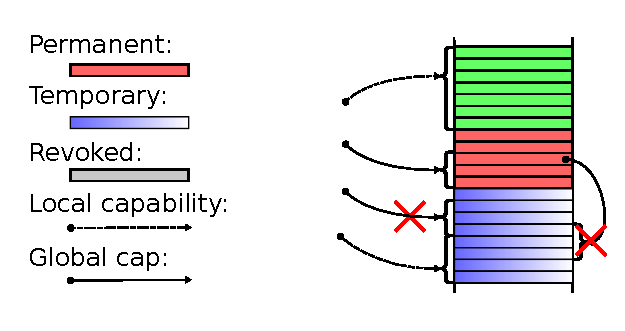
\includegraphics{w11}
  \caption{Illustration of the relation between local and global capabilities and temporary and permanent regions. The table represents a memory and the colored fields are regions governing parts of the memory. Roughly speaking, global capabilities should never depend on memory governed by temporary regions.}
  \label{fig:cap-world}
\end{figure}

\subsubsection{Future worlds}
The future world relations model how memory may evolve over time. 
The \emph{public future world} 
$W' \futurewk W$ is defined to mean that $\dom(W') \supseteq \dom(W)$
and $\forall r \in \dom(W) \ldotp W'(r) \futurewk W(r)$.  That is,
in a public future world, more regions may have been allocated, and
each of the regions may also have evolved according to the public future
region relation (defined below). The \emph{private future world} relation
$W' \futurestr W$ is defined similarly, using a private future region
relation.

The properties of the \emph{private future region} relation are:
\begin{mathpar}
  \inferrule{ (v,\phi_\pub,\phi,H) = (v',\phi_\pub',\phi',H') \\
              (s,s') \in \phi} 
  {  (v',s',\phi_\pub',\phi',H') \futurestr (v,s,\phi_\pub,\phi,H) }
  \and
  \inferrule{ r \in \Regions }
  { r \futurestr (\temp,s,\phi_\pub,\phi,H) }
  \and
  \inferrule{ r \in \Regions }
  { r \futurestr \revoked }
\end{mathpar}
These rules express that, in the private future region relation, we allow
revocation of temporary regions. As explained above, this can be done using a
special revoked region, which does not describe any memory, but we also allow
any other region to serve as a mask, and thus any region $r$ can be a future
region of a temporary region and of a revoked region. On the other hand,
permanent regions cannot be masked away. They are only allowed to take a
transition in the private part of the transition system.

The \emph{public future} region relation satisfies
% \dominique{is defined by?} 
% \lau{As I have understood it, the relation from the theorem defines the future world relations and indirectly the future region relations. It can be shown that these will have the properties mentioned below}
the following properties:
\begin{mathpar}
  \inferrule{ (v,\phi_\pub,\phi,H) = (v',\phi_\pub',\phi',H') \\
    (s,s') \in \phi_\pub }
  {  (v',s',\phi_\pub',\phi',H') \futurewk (v,s,\phi_\pub,\phi,H) }
  \and
  \inferrule{ (\temp,s,\phi_\pub,\phi,H) \in \Regions }
  { (\temp,s,\phi_\pub,\phi,H) \futurewk \revoked }
  \and
  \inferrule{ }
  { \revoked \futurewk \revoked }
\end{mathpar}
In the public future regions we do not permit revocation of temporary regions.
Instead, temporary and permanent regions are only allowed to take a transition
in the public part of the transition system. Revoked regions can either remain
revoked or be masked away by a temporary region. This means that the public
future world relations allows us to reuse a region that has been revoked
earlier.

Notice that the public future region relation is a subset of the
private future region relation.


%%%%%%%%

% In order to model changes to memory over time, we use the future world
% relations. The future world relations model how more memory may be
% allocated but also how memory may change. How memory is allowed to
% change over time depends on the region that governs it and the future
% world relation used. The most interesting part about the future worlds
% is how it affects the regions, so we first look at the properties of
% the \emph{public future region} relation and the \emph{private future
%   region} relation. We then use these relations to describe the future
% world relations.

% {\bf Private future regions}
% In the private future region relation, we allow revocation of $\temp$
% regions. The regions cannot be revoked by removing them from the
% world, because we need the future world relations to be
% monotone. This is why we have the $\revoked$ region, so we have
% a region that can serve as a mask. We can, however, let any region
% serve as a mask, so in the private future region relation, we allow a
% $\temp$ region to become any valid region. As the $\revoked$ region
% serves as a mask, we let any valid region take its place in the
% private future region relation.

% If a $\temp$ region is not masked by a region, then it behaved like a
% $\perm$ region. The $\perma$ regions stay the same type and they are
% allowed to take a transition in the private part of the transition
% system. Which can be thought of as the memory changes according to
% some protocol.

% The properties of the \emph{private future region} relation are:
% \begin{mathpar}
%   \inferrule{  (s,s') \in \phi \\
%     (v,\phi_\pub,\phi,H) = (v',\phi_\pub',\phi',H')}
%   {  (v',s',\phi_\pub',\phi',H') \futurestr (v,s,\phi_\pub,\phi,H) }
%   \and
%   \inferrule{ r \in \Regions }
%   { r \futurestr (\temp,s,\phi_\pub,\phi,H) }
%   \and
%   \inferrule{ r \in \Regions }
%   { r \futurestr \revoked }
% \end{mathpar}

% {\bf Public future regions}
% In the public future regions we do not permit revocation of $\temp$
% regions. In this relation, the $\temp$ and $\perma$ regions must stay
% the same type and they are allowed to take a transition in the public
% part of the transition system.

% The $\revoked$ regions serve as masking regions, but are not as
% liberal as in the private future region relation when it comes to
% letting other regions replace them as masks. In the public future
% region relation, we only allow $\revoked$ and $\temp$ regions to take
% on the job as masking region. We have this limitation, because we
% want the private future region relation to be able to reuse any region
% it has revoked.

% The \emph{public future} region relations satisfies the following properties:
% \begin{mathpar}
%   \inferrule{  (s,s') \in \phi_\pub \\
%     (v,\phi_\pub,\phi,H) = (v',\phi_\pub',\phi',H')}
%   {  (v',s',\phi_\pub',\phi',H') \futurewk (v,s,\phi_\pub,\phi,H) }
%   \and
%   \inferrule{ (\temp,s,\phi_\pub,\phi,H) \in \Regions }
%   { (\temp,s,\phi_\pub,\phi,H) \futurewk \revoked }
%   \and
%   \inferrule{ }
%   { \revoked \futurewk \revoked }
% \end{mathpar}

% Notice that the public future region relation is a subset of the
% private future region relation, so anything you are allowed to do in
% the public future region relation, the private future region relation
% can do the same.


% % The future world relation are really the ones from thm, the above
% % are properties of them.
% {\bf Future world relations}
% There are two future world relations a \emph{public future world}
% relation and a \emph{private future world} relation. In both future
% world relations, we have extension ordering, so a future world $W'$ of
% $W$ has at least the same regions as $W$, but $W'$ may have new regions
% imposing new protocols on parts of the memory. The two future world
% relations differ in the way existing regions are allowed to
% evolve. The public future world relation uses the public future region
% relation and the private future world relation uses the private future
% region relation:
% \begin{mathpar}
%   \inferrule{ \dom(W') \supseteq \dom(W)\\ 
%     \forall r \in \dom(W) \ldotp W'(r) \futurewk W(r) }
%   { W' \futurewk W }
%   \and
%   \inferrule{ \dom(W') \supseteq \dom(W)\\ 
%     \forall r \in \dom(W) \ldotp W'(r) \futurestr W(r) }
%   { W' \futurestr W }
% \end{mathpar}

% % Relate to STSs for high-level languages. Have the public-private
% % transitions, but they are also used for more than this
% \todo[inline]{Relate to STSs for high-level languages?}

\subsubsection{World satisfaction}
A memory satisfies a world, written $\memSat{\ms}{W}$, 
if it can be partitioned into disjoint parts such that each part is
in the interpretation of an active (permanent or temporary) region. 
\begin{align*}
  &\memSat{\ms}{W}
    \text{ iff }\\
  &\quad \left\{\begin{aligned}
        &\exists P : \activeReg{W} \rightarrow \HeapSegments \ldotp \hs = \biguplus_{r\in\activeReg{W}}P(r) \text{\footnotesize{ and }} \\[-.2cm]
        &\quad \forall r \in \activeReg{W} \ldotp \exists H,s \ldotp\\
        &\qquad W(r) = (\_,s,\_,\_,H) \text{\footnotesize{ and }} \npair[n]{P(r)} \in H(s)(\xi^{-1}(W))\\
      \end{aligned}\right.
\end{align*}



\subsection{Logical relation}
\afterpage{
\begin{figure}[htbp]
  \centering
  \begin{withmathindent}{0cm}
    \begin{align*}
      & \observations \; : \;  \Worlds \nefun \UPred{\Regs \times \HeapSegments} \\
      & \observations (W) \defeq \\
      & \;\left\{ \npair{(\reg,\ms)} \; \middle| \;
        \begin{aligned}
          & \forall \ms_f, \heap', i \leq n \ldotp \\
          & (\reg,\ms \uplus \ms_f) \step[i] (\halted,\heap')  \\
          & \;\; \Rightarrow
          \begin{aligned}[t]
            & \exists W' \futurestr W, \ms_r, \ms' \ldotp\\
            & \;\; \heap' = \ms' \uplus \ms_r \uplus \ms_f \text{\footnotesize{ and }} \\
            & \;\; \heapSat[\hs']{n-i}{W'}
          \end{aligned}
        \end{aligned}\right\}\\
      & \stdrr \; : \; \Worlds \monwknefun \UPred{\Regs} \\
      & \stdrr(W) \defeq \left\{ \npair{\reg} \; \middle| \;
          \forall r \in \RegName \setminus \{\pcreg\} \ldotp \npair{\reg(r)}
          \in \stdvr(W) \right\} \\
      & \\[-.2cm]
      & \stder \; : \; \Worlds \nefun \UPred{\Words} \\
      & \stder(W) \defeq \left\{ \npair{\pc} \; \middle| \;
        \begin{multlined}
          \forall n' \leq n, \npair[n']{\reg} \in \stdrr(W), \heapSat[\hs]{n'}{W} \ldotp \\
          \npair[n']{(\reg\update{\pcreg}{\pc},\hs)} \in \observations(W)
        \end{multlined} \right\} \\
      & \\
      &\stdvr \; : \; \Worlds \monwknefun \UPred{\Words} \\
      &\stdvr(W)\defeq  \\
      &\;\;\begin{aligned}[t] & \{ \npair{i} \mid i \in \ints \}
        \union \\
        & \{ \npair{\stdcap[(\noperm,\gl)] } \}
        \union \\
        & \left\{
          \begin{multlined}
            \npair{\stdcap[(\readonly,\gl)] } \mid \\
            \npair{(\start,\addrend)} \in \readCond{}(\gl)(W)
          \end{multlined} \right\}
        \union \\
        & \left\{
          \begin{aligned}
            &\npair{\stdcap[(\readwrite,\gl)] } \mid \\
             &\quad\npair{(\start,\addrend)} \in \readCond{}(\gl)(W) \text{\footnotesize{ and }} \\
             &\quad\npair{(\start,\addrend)} \in
            \writeCond{}(\iota^\nwl,\gl)(W)
          \end{aligned} \right\} \union \\
        & \left\{
          \begin{aligned}
            &\npair{\stdcap[(\readwritel,\gl)] } \mid \\
             &\quad\npair{(\start,\addrend)} \in \readCond{}(\gl)(W) \text{\footnotesize{ and }} \\
             &\quad\npair{(\start,\addrend)} \in
            \writeCond{}(\iota^\pwl,\gl)(W)
          \end{aligned} \right\}
        \union \\
        & \left\{
          \begin{aligned}
            &\npair{\stdcap[(\exec,\gl)]} \mid \\
             &\quad\npair{(\start,\addrend)} \in \readCond{}(\gl)(W) \text{\footnotesize{ and }} \\
             &\quad\npair{(\{\exec\},\start,\addrend)} \in \execCond{}(\gl)(W)
          \end{aligned} \right\}
        \union \\
        & \left\{
          \begin{multlined}
            \npair{\stdcap[(\entry,\gl)]} \mid \\
            \npair{(\start,\addrend,\addr)} \in \entryCond{}(\gl)(W)
          \end{multlined} \right\}
        \union \\
        & \left\{
          \begin{aligned}
            &\npair{\stdcap[(\rwx,\gl)]} \mid \\
            &\quad\npair{(\start,\addrend)} \in \readCond{}(\gl)(W) \text{\footnotesize{ and }} \\
            &\quad\npair{(\start,\addrend)} \in \writeCond{}(\iota^\nwl,\gl)(W) \text{\footnotesize{ and }}\\
            &\quad\npair{(\{\rwx,\exec\},\start,\addrend)} \in \execCond{}(\gl)(W)
          \end{aligned} \right\}
        \union \\
        & \left\{
          \begin{aligned}
            &\npair{\stdcap[(\rwlx,\gl)]} \mid \\
             &\quad\npair{(\start,\addrend)} \in \readCond{}(\gl)(W) \text{\footnotesize{ and }} \\
             &\quad\npair{(\start,\addrend)} \in \writeCond{}(\iota^\pwl,\gl)(W) \text{\footnotesize{ and }}\\
             &\quad\npair{(\{\rwlx,\rwx,\exec\},\start,\addrend)} \in
            \execCond{}(\gl)(W)
          \end{aligned} \right\}
      \end{aligned}
    \end{align*}
  \end{withmathindent}
  \caption{Logical Relation}
  \label{fig:logrel}            
\end{figure}


% \begin{figure}[htbp]
%   \centering
%   \begin{align*}
%   &\iota_{\start,\addrend}^\pwl : \Regions\\
%   &\iota_{\start,\addrend}^\pwl \defeq (\temp,1,=,=,H^\pwl_{\start,\addrend}) \\
%   \\
%   &H^\pwl : \Addrs^2 \fun \States \fun (\Wor \monwknefun \UPred{\HeapSegments})\\
%   &H^\pwl_{\start,\addrend}\; s \; \hat{W} \defeq  \quad\left\{\npair{\hs} \; \middle| \;
%     \begin{aligned}
%       & n = 0 \text{\footnotesize{ or }} (\dom(\hs) = [\start,\addrend] \text{\footnotesize{ and }} \\
%       &\forall \addr \in [\start,\addrend] \ldotp\\
%       & \;\; \npair[n-1]{\hs(\addr)} \in \stdvr(\xi(\hat{W})))
%     \end{aligned}
%         \right\}\\
%   &\iota_{\start,\addrend}^{\nwl} : \Regions \\
%   &\iota_{\start,\addrend}^{\nwl} \defeq (\temp,1,=,=,H^\nwl_{start,\addrend}) \\
%   \\
%   &H^\nwl : \Addrs^2 \fun \States \fun (\Wor \monstrnefun \UPred{\HeapSegments})\\
%   &H^\nwl_{\start,\addrend} \; s \;\hat{W} \defeq \quad\left\{\npair{\hs} \; \middle| \;
%     \begin{aligned}
%       &n = 0 \text{\footnotesize{ or }} (\dom(\hs) = [\start,\addrend] \text{\footnotesize{ and }}\\
%       &\forall \addr \in [\start,\addrend] \ldotp \\
%       & \;\; {\footnotesize\nonlocal{\ms(\addr)}} \text{\footnotesize{ and }}\\
%       & \;\; \npair[n-1]{\hs(\addr)} \in \stdvr(\xi(\hat{W})))
%      \end{aligned}
%      \right\}
% \end{align*}
% \caption{Standard regions}
% \label{fig:standard-regions}
% \end{figure}


\begin{figure}[htbp]
  \centering
  \begin{align*}
  & \readCond{}(\gl)(W) =  \\
  & \left\{ \npair{(\start,\addrend)} \; \middle| \;
    \begin{aligned}
      & \exists r \in \var{localityReg}(g,W) \ldotp \\
      & \;\; \exists [\start',\addrend'] \supseteq [\start,\addrend] \ldotp W(r)\nsubsim[n] \iota_{\start',\addrend'}^\pwl 
    \end{aligned} \right\}\\
  & \writeCond{}(\iota,\gl)(W) =  \\
  & \left\{
    \npair{(\start,\addrend)}
    \; \middle| \;
    \begin{aligned}
      & \exists r \in \var{localityReg}(g,W) \ldotp \\
      & \;\; W(r) \text{\footnotesize{ is address-stratified and}} \\
      & \;\; \exists [\start',\addrend'] \supseteq [\start,\addrend] \ldotp W(r)\nsupsim[n-1] \iota_{\start',\addrend'}
    \end{aligned} \right\}\\
  & \execCond{}(\gl)(W) = \\
  & \left\{
    \begin{multlined}
      \npairP{(\var{perms}, \\
        \start,\addrend)}
    \end{multlined}
     \; \middle| \;
    \begin{aligned}
      & \forall n' < n, W' \future W, a \in [\start,\addrend], \perm \in \var{perms} \ldotp \\
      & \;\;\;\; \npair[n']{((\perm,\gl),\start,\addrend,\addr)} \in \stder(W')\\
    \end{aligned} \right\} \\
  & \entryCond{}(\gl)(W) = \\
  & \left\{ \npair{(\start,\addrend,\addr)} \; \middle| \;
    \begin{aligned}
 &  \forall n' < n \ldotp \forall W' \future W \ldotp\\
      & \quad \npair[n']{((\exec,\gl),\start,\addrend,\addr)} \in \stder(W')
    \end{aligned} \right\} \\
  & \quad \text{where } \gl = \local \Rightarrow \future = \futurewk \\
  & \quad \text{and } \gl = \glob \Rightarrow \future = \futurestr
  \end{align*}
\caption{Permission-based conditions}
\label{fig:perm-conds}
\end{figure}
}
%subsection introduction
% \dominique{I would try to motivate the LR defs by saying that the LR is
%   constructed to express the FTLR and the FTLR says that if a piece of code only
%   has access to values respecting the invariants in a world, then it will
%   respect them itself too.} 
The logical relation defines semantically what it
means to be capability safe.
% \dominique{We have not introduced capability
%   safety..} 
In large parts, capability safety is defined by when a capability
can be safely given to an adveserial piece of code. In the following paragraphs,
we will go through the definitions of the logical relation and provide an
intuition why they define capability safety. The definition of the logical
relation is found in \figurename~\ref{fig:logrel}, and \figurename~\ref{fig:perm-conds}.
Some definitions are omitted and explained when needed. The precise definitions
can be found in the technical appendix~\cite{technical_appendix}.

The \emph{observation relation} $\observations$ defines which configurations
are capability safe. Roughly speaking, a configuration is capability safe if,
whenever it halts, then the resulting memory satisfies a private future world.
Notice that failing is considered safe behavior and in fact, the machine will
often resort to failing when, for example, an unauthorized
access is attempted, like a load of a memory location through a
capability without read permission. This is similar to the logical relation
given for an untyped language in~\cite{Devriese:2016ObjCap}, but unlike logical
relations for typed languages, which typically require that computations do not
fail.

The \emph{register-file relation} $\stdrr$ specifies that register-files are
safe when they contain safe words (i.e.\ words in $\stdvr$) in all registers but
$\pcreg$. The \emph{expression relation} $\stder$ defines when a word is safe
to use as a program counter. That is the case when the word can be plugged into
a capability safe register file (i.e.\ a register file in $\stdrr$) and paired
with a memory satisfying the world to become a capability safe configuration.

The \emph{value relation} $\stdvr$ defines when words are safe, i.e.\ when they
cannot be used to break the protocols defined by the world. Non-capability data
is always safe because it provides no authority. Capabilities give the authority
to manipulate memory and potentially break memory protocols, so they need to
satisfy certain conditions to be capability safe. In
\figurename~\ref{fig:perm-conds}, we define such a condition for each kind of
permission a capability can have (we will call these permission-based
conditions).

For capabilities with read permission, the $\readCond{}$ ensures that it can
only be used to read capability safe words, by requiring that the region
governing the relevant part of memory, guarantees that the memory contains only
words in the value relation. Generally speaking, global capabilities should only
depend on permanent regions. Therefore we use the function
$\var{localityReg}(\gl,W)$, which projects out all active regions when
$\gl$ (the locality) is local, but only the permanent regions when $\gl$ is global.
The read condition is defined in terms of a standard region
$\iota^\pwl_{\start,\addrend}$ which requires all the words in the range
$[\start,\addrend]$ to be safe.

For a capability with write permission, $\writeCond{}$ must be
satisfied for the capability's range of authority. Such a capability
may be used to write any word, so the region governing the relevant
part of memory must (at least) allow any capability safe word to be
stored. However, this is not entirely true because of the distinction
between write and permit-write-local capabilities.  Only
permit-write-local capabilities need to allow arbitrary safe values to
be stored, while for write capabilities, it is sufficient to allow
storing values that are both non-local and safe. The write condition
uses $\var{localityReg}$ to pick an appropriate region for its
locality in the same way the read condition does. The condition for
the region to be address-stratified is there for technical reasons and for the full definition, we refer to the technical appendix. In
the value relation, the write condition is used with $\iota^\pwl$ for
write-local capabilities. For write capabilities, the write condition
is used with another standard region $\iota^\nwl_{\start,\addrend}$
which requires all the words in the range $[\start,\addrend]$ to be
non-local and safe.

The conditions $\entryCond{}$ and $\execCond{}$ are very similar and differ only
slightly. In both cases, we require that the capability can be safely jumped to.
However, executable capabilities can be updated to point anywhere in memory, so
they must be capability safe as a program counter (in the $\stder$-relation) no
matter where they point to. In contrast, enter capabilities are opaque and can
only be used to jump to the address they point to. They also change permission
when jumped to, so we require them to be capability safe as a program counter
when the permission is changed to read/execute. Because the capabilities are not
necessarily invoked immediately, we need to require that this is the case in a
future world, but it depends on the locality of the capability which future
worlds we consider. If the capability is global, then it should only depend on
permanent regions, so we require capability safety as a program counter in any
\emph{private} future world (recall that temporary regions may be revoked in a
private future world). For local capabilities, it suffices to be capability safe
in \emph{public} future worlds, where temporary regions are still there.

\subsection{Safety of the capability machine}
With the logical relation defined, we can now state the fundamental theorem of
our logical relation: a strong theorem that formalises the guarantees offered by
the capability machine. Essentially, it says that a capability that only grants
safe authority is capability safe as a program counter.
\begin{theorem}[Fundamental Theorem]
  \label{thm:ftlr}
  If one of the following holds:
  \begin{align*}
      & \bullet
        \begin{aligned}[t]
        &\perm = \exec \text{\footnotesize{ and }}\npair{(\start,\addrend)} \in \readCond{}(\gl)(W)
      \end{aligned} \\
    & \bullet 
      \begin{aligned}[t]
        &\perm = \rwx \text{\footnotesize{ and }} \\
        &\npair{(\start,\addrend)} \in \readCond{}(\gl)(W) \text{\footnotesize{ and }}\\
        &\npair{(\start,\addrend)} \in \writeCond{}(\iota^\nwl,\gl)(W)
      \end{aligned} \\
    & \bullet 
      \begin{aligned}[t]
        &\perm = \rwlx \text{\footnotesize{ and }}\\
        &\npair{(\start,\addrend)} \in \readCond{}(\gl)(W) \text{\footnotesize{ and }}\\
        &\npair{(\start,\addrend)} \in \writeCond{}(\iota^\pwl,\gl)(W),
      \end{aligned}
  \end{align*}
  then $\npair{((\perm,\gl),\start,\addrend,\addr)} \in \stder(W)$
\end{theorem}
The Fundamental Theorem allows us to prove capability safety for
adveserial programs: if the authority granted by
the capabilty for the untrustred program is reasonable, then it is safe to
execute. Intuitively, this is because our logical relation captures the
safe behaviours of the capability machine that do not allow you to
produce something \emph{unsafe} from something safe. 
The Fundamental Theorem also serves as a sanity check of the
logical relation as it guarantees that a large class of capabilities
actually inhabits it.

\section{Examples}
\label{sec:examples}
In this section, we demonstrate how our formal model of capability
safety allows us to prove local state encapsulation and control-flow
correctness properties for challenging program examples. The security
measures of Section~\ref{sec:stack-and-return-pointer} are deployed to
ensure these properties. Since we are dealing with assembly language,
there are many details to the formal treatment, and therefore we
necessarily have to omit some details in the lemmas we state here.
The interested reader can find all the technical details in the
technical appendix~\cite{technical_appendix}.

\subsection{Encapsulation of local state}
The capability machine provides encapsulation of local state. The programs
\texttt{\footnotesize{f1}} and \texttt{\footnotesize{f2}} in
\figurename~\ref{fig:prog-f1-and-f2} demonstrate this. They are very similar: both
store some local state, call an untrusted piece of code ($\adv$), and then test
whether the local state is unchanged. They differ in the way they do this.
Program \texttt{\footnotesize{f1}} assumes it has access to a stack pointer and uses the stack
to store its local state. It also uses the stack-based calling convention
\texttt{\footnotesize{scall}} to call the adversary. On the other hand, \texttt{\footnotesize{f2}} uses
malloc to allocate memory for its local state and uses an activation-record
based calling convention (described in the technical appendix) to run the
adversarial code.

\begin{figure}[t]
  \centering

  \begin{minipage}[t]{4.1cm}
  \begin{lstlisting}
f1: push 1
    fetch $r_1$ $\adv$
    scall $r_1$($[]$,$[]$)
    pop $r_1$
    assert $r_1$ 1
    halt
  \end{lstlisting}
  \end{minipage}
  \begin{minipage}[t]{4.1cm}
  \begin{lstlisting}
f2: malloc $r_l$ 1
    store $r_l$ 1
    fetch $r_1$ $\adv$
    call $r_1$($[]$,$[r_l]$)
    assert $r_l$ 1
    halt
  \end{lstlisting}
  \end{minipage}
  \caption{Two simple programs that rely on local-state encapsulation. \texttt{f1} uses our stack-based calling convention. \texttt{f2} uses a calling not reliant on the stack}
  \label{fig:prog-f1-and-f2}
\end{figure}

For both programs, we can prove that if they are linked with an
adversary, $\adv$, that is allowed to allocate new memory but
otherwise has no capabilities, then the assertion will never fail when
executing the program (see Lemmas~\ref{lem:correctness-f1}
and~\ref{lem:correctness-f2} below).
% \lars{shouldn't we say already
% here that the adversary is a global capability and that is why,
% intuitively, the local state is preserved ?} \lau{Due to the ``order
% of control'', \texttt{f1} runs first. The lemma is quite restrictive
% on the adversary in the sense that it only has access to malloc (and
% whatever we give et access to). Specifically, it does not have access
% to the stack pointer and because of that we don't need to check it
% first. We could write that the lemmas are limited in their assumptions
% to make them simpler and a more complicated example is coming up.}
The two examples also illustrate the versatility of the logical relation.
Because it is not specific to any calling convention, we can use it to reason
about both programs, even though they use different calling conventions.


% \begin{lemma}[Correctness lemma for \texttt{f1}]
% \todo[inline]{The lemma copied directly from the TR. To be deleted later!}
%   \label{lem:correctness-f1}
%   Let
%   \begin{align*}
%     c_{\var{adv}} & \defeq ((\entry,\glob),\start_{\adv},\addrend_{\adv},\start_{\adv}+\olf) \\
%     c_{f1} & \defeq ((\rwx,\glob),\mathtt{f1}-\olf,\mathtt{1f},\mathtt{f1}) \\
%     c_\malloc & \defeq ((\entry,\glob),\start_\malloc,\addrend_\malloc,\start_\malloc+\olf) \\
%     c_{\var{stk}} & \defeq ((\rwlx,\local),\start_\stk,\addrend_\stk,\start_\stk-1) \\
%     c_\link & \defeq ((\readonly,\glob),\link,\link+1,\link)\\
%     \reg & \in \Regs \\
%     m & \defeq \hs_{f1} \uplus 
%         \hs_\flag \uplus                
%         \ms_{\var{link}} \uplus 
%         \hs_\adv \uplus 
%         \ms_{\malloc} \uplus 
%         \ms_{\var{stk}} \uplus
%         \ms_{\var{frame}} 
%   \end{align*}
%   and
%   \begin{itemize}
%   \item $c_\malloc$ satisfies the specification for malloc and $\iota_{\malloc,0}$ is the region from the specification.
%   \end{itemize}
%   where 
%   \begin{align*}
%     &\dom(\hs_{f1}) = [\mathtt{f1}-\olf,\mathtt{1f}] \\
%     &\dom(\hs_\flag) = [\flag,\flag] \\
%     &\dom(\ms_\link) = [\link,\link+1]\\
%     &\dom(\ms_\stk) = [\start_\stk, \addrend_\stk]\\
%     &\dom(\hs_{\adv}) = [\start_\adv,\addrend_\adv] \\
%     &\heapSat[\hs_{\malloc}]{n}{[0 \mapsto \iota_{\malloc,0}]} \qquad \text{ for all $n \in \nats$}
%   \end{align*}
%   and
%   \begin{itemize}
%   \item $\ms_{f1}(\mathtt{f1}-\olf) = ((\readonly,\glob),\link,\link+1,\link)$, $\ms_{f1}(\mathtt{f1}-\olf+1) = ((\readwrite,\glob),\flag,\flag,\flag)$, the rest of $\hs_{f1}$ contains the code of $f1$.
%   \item $\ms_\flag = [\flag \mapsto 0]$
%   \item $\ms_{\var{link}} = [\var{link} \mapsto c_\malloc, \var{link} + 1 \mapsto c_\adv]$
%   \item $\hs_\adv(\start_\adv) = c_\link$ and $\forall \addr \in [\start_\adv+1,\addrend]\ldotp \ms_\adv(a) \in \ints$
%   \end{itemize}
%   if 
%   \[
%     (\reg\update{\pcreg}{c_{f1}}\update{r_\stk}{c_\stk},m) \step[n] (\halted,m'),
%   \]
%   then
%   \[
%     m'(\flag) = 0
%   \]  
% \end{lemma}


In order to formulate lemmas about \texttt{\footnotesize{f1}} and \texttt{\footnotesize{f2}}, we
need a way to observe whether the assertion fails. To this end, we
assume access to a flag (an address in memory). When the assertion
fails, it sets the flag to $1$ and halts. A slightly simplified
version of the correctness lemma for \texttt{\footnotesize{f1}} is:
\begin{lemma}
  \label{lem:correctness-f1}
  Let
\[
    \begin{array}{r@{}lr@{}l}
    c_{\var{adv}} & \;\defeq ((\entry,\glob),\dots) & c_{\var{stk}} & \;\defeq ((\rwlx,\local),\dots)\\
    c_{f1} & \;\defeq ((\rwx,\glob),\dots) & c_\link &\; \defeq ((\readonly,\glob),\dots)\\
    c_\malloc &\; \defeq ((\entry,\glob),\dots) & \reg& \; \in \Regs \\
    m &  \multicolumn{3}{@{}l}{\;\defeq \ms_{f1} \uplus \ms_\flag \uplus \ms_{\var{link}} \uplus \hs_\adv \uplus \ms_{\malloc} \uplus} \\
      & \multicolumn{3}{@{}l}{\phantom{\;\defeq \;}  \ms_{\var{stk}} \uplus \ms_{\var{frame}}} \\
    \end{array}
\]
  where each of the capabilities have an appropriate range of authority and pointer. Furthermore
  \begin{itemize}
  \item $\ms_{f1}$ contains $c_\link$, $c_\flag$ and the code of \texttt{\footnotesize{f1}}
  \item $\ms_\flag(\flag) = 0$
  \item $\ms_{\var{link}}$ contains $c_\adv$ and $c_\malloc$
  \item $\hs_\adv$ contains $c_\link$ and otherwise only instructions.
  \end{itemize}
  If $(\reg\update{\pcreg}{c_{f1}}\update{r_\stk}{c_\stk},m) \step^* (\halted,m')$,
  then $m'(\flag) = 0$
\end{lemma}

To prove Lemma~\ref{lem:correctness-f1}, it suffices to show that the start
configuration is capability safe (in the $\observations$ relation) for a world
with a permanent region that requires the assertion flag to be 0. We prove this
using an anti-reduction lemma by which it suffices to show that the
configuration is capability safe after some reduction steps. We then use a general lemma
for reasoning about \texttt{\footnotesize{scall}}, by which it suffices to show that (1) the
configuration that \texttt{\footnotesize{scall}} will jump to is capability safe and (2) that
the configuration just after \texttt{\footnotesize{scall}} is done cleaning up is capability
safe. We use the Fundamental Theorem to reason about the unknown code, but
notice that the Fundamental Theorem says nothing about enter capabilities and
that the adversary capability is an enter capability. Luckily the enter
capability becomes $\exec$ after the jump and then, the Fundamental Theorem
applies.

We have a similar lemma for \texttt{\footnotesize{f2}}:
\begin{lemma}
  \label{lem:correctness-f2}
  Making similar assumptions about capabilities and linking as in
  Lemma~\ref{lem:correctness-f1} but assuming no stack pointer
  if $(\reg\update{\pcreg}{c_{f2}},m) \step^* (\halted,m')$, then $m'(\flag) = 0$.
\end{lemma}

\subsection{Well-bracketed control-flow} 
Using the stack-based calling convention of \texttt{\footnotesize{scall}}, we get
well-bracketed control-flow. To illustrate this, we look at
two example programs \texttt{\footnotesize{f3}} and
\texttt{\footnotesize{g1}} in \figurename~\ref{fig:prog-f3-and-g1}.

In \texttt{\footnotesize{f3}} there are two calls to an adversary and in order for the
assertion in the middle to succeed, they need to be well-bracketed. If the
adversary was able to store the return pointer from the first call and invoke
it in the second call, then \texttt{\footnotesize{f3}} would have $2$ on top of its stack and
the assertion will fail. However, the security measures of our calling
convention explained in Section~\ref{sec:stack-and-return-pointer} prevent this
sort of attack: specifically, the return pointer is local, so it can only be
stored on the stack, but the part of the stack that is accessible to the
adversary is cleared before the second invocation. The following lemma shows
that there are also no other attacks that will break well-bracketedness of this
example, i.e.\ the assertion never fails. It is similar to the two previous
lemmas:

\begin{comment}
\newsavebox{\testit}
\begin{lrbox}{\testit}
  \begin{lstlisting}
g1:  malloc $r_2$ 1
     store $r_2$ 0
     move $\pcreg$ $r_3$
     lea $r_3$ $\var{offset}$
     crtcls $[(x, r_2)]$ $r_3$
     rclear $\RegName \setminus \{\pcreg,r_0,r_1 \}$
     jmp $r_0$
f4:  reqglob $r_1$
     prepstk $r_\stk$
     store $x$ 0
     scall $r_1$($[]$,$[r_0,r_1,r_{\var{env}}]$)
     store $x$ 1
     scall $r_1$($[]$,$[r_0,r_{\var{env}}]$)
     load $r_1$ $x$
     assert $r_1$ 1
     mclear $r_\stk$
     rclear $\RegName \setminus \{r_0,\pcreg\}$
     jmp $r_0$
\end{lstlisting}
\end{lrbox}

\newsavebox{\progfthree}
\begin{lrbox}{\progfthree}
  \begin{lstlisting}
f3: push 1
    fetch $r_1$ $\adv$
    scall $r_1$($[]$,$[r_1]$)
    pop $r_2$
    assert $r_2$ 1
    push 2
    scall $r_1$($[]$,$[]$)
    halt
\end{lstlisting}
\end{lrbox}

\begin{figure}[t]
  \centering
  \subfloat{\usebox{\testit}}
  \subfloat{\usebox{\progfthree}}
  \caption{test}
\end{figure}
\end{comment}
\begin{figure}[t]
  \centering
  \begin{minipage}[t]{5.05cm}
  \begin{lstlisting}
g1:  malloc $r_2$ 1
     store $r_2$ 0
     move $\pcreg$ $r_3$
     lea $r_3$ $\var{offset}$
     crtcls $[(x, r_2)]$ $r_3$
     rclear $\RegName \setminus \{\pcreg,r_0,r_1 \}$
     jmp $r_0$
f4:  reqglob $r_1$
     prepstk $r_\stk$
     store $x$ 0
     scall $r_1$($[]$,$[r_0,r_1,r_{\var{env}}]$)
     store $x$ 1
     scall $r_1$($[]$,$[r_0,r_{\var{env}}]$)
     load $r_1$ $x$
     assert $r_1$ 1
     mclear $r_\stk$
     rclear $\RegName \setminus \{r_0,\pcreg\}$
     jmp $r_0$
\end{lstlisting}
  \end{minipage}
  \begin{minipage}[t]{3.4cm}
  \begin{lstlisting}
f3: push 1
    fetch $r_1$ $\adv$
    scall $r_1$($[]$,$[r_1]$)
    pop $r_2$
    assert $r_2$ 1
    push 2
    scall $r_1$($[]$,$[]$)
    halt
\end{lstlisting}
  \end{minipage}
  \caption{ Two programs that rely on well-bracketedness of
    \texttt{scall}s to function correctly. $\var{offset}$ is the
    offset to \texttt{f4}.}
  \label{fig:prog-f3-and-g1}
\end{figure}

\begin{lemma}
  \label{lem:correctness-f3}
  Making similar assumptions about capabilities and linking as in
  Lemma~\ref{lem:correctness-f1}
  if $(\reg\update{\pcreg}{c_{f3}}\update{r_\stk}{c_\stk},m) \step^*
  (\halted,m')$, then $m'(\flag) = 0$.
\end{lemma}

The final example, \texttt{\footnotesize{g1}} with \texttt{\footnotesize{f4}}, is a faithful translation
of a tricky example known from the
literature~\citep{pitts_operational_1998,Dreyer:jfp12}. It consists of two
parts, \texttt{\footnotesize{g1}} and \texttt{\footnotesize{f4}}. \texttt{\footnotesize{g1}} is a closure generator that
generates closures with one variable $x$ set to $0$ in its environment and
\texttt{\footnotesize{f4}} as the program. \texttt{\footnotesize{f4}} expects one argument, a callback. The
program sets $x$ to $0$ and calls the callback. When it returns, \texttt{\footnotesize{f4}}
sets $x$ to $1$ and calls the callback a second time. When it returns from the
callback, it asserts that $x$ is $1$ and returns. This example is more
complicated than the previous ones because it involves a closure invoked by the
adversary and an adversary callback invoked by us. As explained in
Section~\ref{sec:stack-and-return-pointer}, this means we need to (1) take care
to properly check the stack pointer received by our closure from the adversary
(it must have the correct permission and fit with our calling convention) and (2)
require that the adversary callback is global.

To illustrate how subtle this program is, consider how an adversary could try to
make the assertion fail. In the second callback an adversary can get to the
first callback by invoking the closure one more time. If there were any way for
the adversary to transfer the return pointer from the point where it reinvokes
the closure to where the closure reinvokes the callback, then the assertion can
be made to fail. Similarly, if there were any way for the adversary to store a
stack pointer or trick the trusted code into preserving it across an invocation,
the assertion can likely be made to fail too. However, our calling convention
guarantees that there is no way any of this can happen, as we prove in the
following lemma.

\begin{lemma}
  \label{lem:correctness-g1}
  Let
\[
    \begin{array}{r@{}lr@{}l}
    c_{\var{adv}} & \;\defeq ((\rwx,\glob),\dots) & c_{g1} & \;\defeq ((\entry,\glob),\dots)
    \end{array}
\]
  and otherwise make assumptions about capabilities and linking similar to Lemma~\ref{lem:correctness-f1} 
  if
  \[
  (\reg_0\update{\pcreg}{c_\adv}\update{r_\stk}{c_\stk}\update{r_1}{c_{g1}},m) \step^* (\halted,m'),
  \]
  then $m'(\flag) = 0$.
\end{lemma}

As explained in Section~\ref{sec:stack-and-return-pointer}, the callback must be
global, essentially to make sure that it is not allocated on the stack where it
might contain the adversary's original stack pointer. If not, it could break the
encapsulation of our local stack frame. In the proof of
Lemma~\ref{lem:correctness-g1}, this requirement shows up because we invoke the
callback in a world that is only a private future world of the one where we
received the callback, precisely because we have invalidated the local state of
the adversary (particularly its previous stack and return capabilities). The
callback is still valid in this private future world, but only because we know
that it is global.

In Lemma~\ref{lem:correctness-g1} the order of control has been inverted
compared to the previous lemmas. In this lemma, the adversary assumes control
first with a capability for the closure creator \texttt{\footnotesize{g1}}. This means we need
to check that all arguments are safe to use and that we clean up before
returning in the end. The inversion of control poses an interesting challenge
when it comes to reasoning about the adversary's local state during the
execution of \texttt{\footnotesize{f4}}. During the execution of \texttt{\footnotesize{f4}} and the callbacks,
the adversary should not be able to rely on its local state from before the call
of \texttt{\footnotesize{f4}}. This is easily done by revoking all the temporary regions of the
world given at the start of \texttt{\footnotesize{f4}}. However, when \texttt{\footnotesize{f4}} returns, the
adversary is again allowed to rely on its old local state which means that we
need to guarantee that the local state is unchanged. This is important because
the return pointer that \texttt{\footnotesize{f4}} receives from the adversary may be local,
and the adversary is allowed to allocate the activation record on the stack
(just like we do) so that they can store and recover his old stack pointer after
\texttt{\footnotesize{f4}} returns.

In Figure~\ref{fig:worlds-in-pf-g1}, we illustrate how we accomodate this in the
proof of Lemma~\ref{lem:correctness-g1} by constructing appropriate worlds for
all the situations where control is passed to the adversary. The potentially
local return pointer received by \texttt{\footnotesize{f4}} from the adversary is safe in
$W_1$, so it can only be used in public future worlds. Let us see how $W_6$ is
constructed as a public future world. The worlds $W_2$ and $W_4$ are constructed
by revoking all temporary regions and adding a $\iota^\pwl$ region for the stack
we pass away and static temporary regions (a region that accepts exactly one
memory) for our local stack as well as the adversary's local stack. The given
worlds $W_3$ and $W_5$ are public future worlds in which the adversary chooses
to return to us. None of these worlds can have masked the temporary regions of
$W_1$ with permanent regions. $W_6$ is constructed by revoking the temporary
regions of $W_5$ and reinstating the temporary regions of $W_1$. This makes
$W_6$ a public future world of $W_1$. It is therefore safe to use the return
pointer to return to the adversary, since we have restored validity of any local
state they might have stashed away.

\begin{figure}[t]
  \centering
\begin{tikzpicture}[main node/.style={}, node distance=1.5cm]
  \node[main node] (1) {$W_1$};
  \node[main node] (label1) [below of=1,yshift=1cm] {\footnotesize{\textit{\texttt{f3} called}}};
  \node[main node,left] (given) [left of=1,yshift=0.05cm] {\parbox{1.5cm}{\footnotesize{Given:}}};

  \node[main node] (2) [above right of=1]{$W_2$};
  \node[main node] (label2) [above of=2,yshift=-1cm] {\textit{\footnotesize{first callback}}};

  \node[main node,left] (const) [above of=given,yshift=-0.4cm] {\parbox{1.5cm}{\footnotesize{Constructed:}}};

  \node[main node] (3) [below right of=2]{$W_3$};
  \node[main node] (label3) [below of=3,yshift=0.75cm] {\footnotesize{\textit{callback returns}}};

  \node[main node] (4) [above right of=3]{$W_4$};
  \node[main node] (label4) [above of=4,yshift=-0.75cm] {\footnotesize{\textit{second callback}}};

  \node[main node] (5) [below right of=4]{$W_5$};
  \node[main node] (label5) [below of=5,yshift=1cm] {\footnotesize{\textit{callback returns}}};

  \node[main node] (6) [above right of=5]{$W_6$};
  \node[main node] (label6) [above of=6,yshift=-1cm] {\footnotesize{\textit{\texttt{f3} returns}}};
  \path(1) edge[draw=none] node [sloped, auto=false, allow upside down] {$\sqsubseteq^\priv$} (2)
       (2) edge[draw=none] node [sloped, auto=false, allow upside down] {$\sqsubseteq^\pub$} (3)
       (3) edge[draw=none] node [sloped, auto=false, allow upside down] {$\sqsubseteq^\priv$} (4)
       (4) edge[draw=none] node [sloped, auto=false, allow upside down] {$\sqsubseteq^\pub$} (5)
       (5) edge[draw=none] node [sloped, auto=false, allow upside down] {$\sqsubseteq^\priv$} (6);
\end{tikzpicture}
  \caption{Illustration of some of the worlds in the proof of
    Lemma~\ref{lem:correctness-g1}. The first row of worlds are worlds
  we construct during the proof. The second row of worlds are worlds
  we are given during the proof. $W_6$ is constructed such that $W_6
  \futurewk W_1$.}
  \label{fig:worlds-in-pf-g1}
\end{figure}
\begin{comment}
\begin{itemize}
\item Ticket dispenser
\item The awkward example and variants
\item A sandboxing example?

For example, an untrusted advertisement scenario with initialization code
that registers a redraw callback. The redraw callback gets temporary
read-write access to a framebuffer.

\item Some compartmentalisation result?
\end{itemize}
\end{comment}

\section{Discussion}
\label{sec:discussion}
\noindent\textbf{Calling convention}\\
\emph{Formulating control flow correctness} While we claim that our calling convention enforces control-flow
correctness, we do not prove a general theorem that shows this, it is not clear what such a theorem should state. Formulations in terms of a control-flow graph, like the one by
\cite{abadi_control-flow_2005}, do not take into account temporal properties,
like the well-bracketedness that Example~\texttt{\footnotesize{g1}} relies on.
In fact, our examples show that our logical relation imply a form of
control-flow correctness that is stronger than such formulations, although this
is not made very explicit. As future work, we consider looking at a more
explicit and useful way to formalise well-bracketed control flow. The idea would
be to define a variant of our capability machine with built-in call and return
instructions and well-bracketed control flow built-in to the operational
semantics, and then prove that compiling such code to our machine using our
calling convention is fully abstract~\cite{abadi_protection_1998}.

\emph{Performance and the requirement for stack clearing} 
The additional security measures of the calling convention described in
Section~\ref{sec:stack-and-return-pointer} impose an overhead compared to
a calling convention that does not provide security. However, the security measures generally consist of a
few checks or register clearings on every boundary crossing between trusted code
and adversary, which should impose an acceptable performance overhead. The only
exception is the requirements for stack clearing which we occur in two
situations: when returning to the adversary and when invoking an adversary
callback. As we have explained, it is not sufficient to clear just the part of
the stack that we have used ourselves, but we need to clear all of the stack that we are not using ourselves. 
In other words on every boundary cross between trusted code and adversary code, a potentially large region of memory must be erased.
We believe this is a common requirement for typical usage scenarios of local capabilities and
capability machines like CHERI should consider to provide special support for
this requirement, in the form of a highly-optimized instruction for erasing
a large block of memory.

\emph{Modularity} It is important that our calling convention is modular.
This means that the requirements we have on callbacks, return
pointers etc. provided to trusted code by an adversary are also satisfied by
callbacks, return pointers etc. that we construct ourselves. For example, our
return pointers are local capabilities because they must point to
memory where we can store the old stack pointer, but the adversary's return
pointers are also allowed to be local. Adversary callbacks on the other hand are
required to be global but the callbacks we construct ourselves are also
allocated on the heap and global. In other words, we do not assume that our code
has some sort of special status and it is possible for the adversary to protect
themselves against us the same way we protect against them.
\\\\
\noindent\textbf{Logical relation}\\
\emph{Single orthogonal closure} The definitions of $\stder$ and $\stdvr$ in
Figure~\ref{fig:logrel} apply a single orthogonal closure, a new variant of an
existing pattern called biorthogonality. Biorthogonality is a pattern for
defining logical relations~\citep{krivine_classical_1994,pitts_operational_1998}
in terms of an observation relation of safe configurations (like we do). The
idea is to define safe evaluation contexts as the set of contexts that produce
safe observations when plugging safe values and define safe terms as the set of
terms that can be plugged into safe evaluation contexts to produce safe values.
This is an alternative to more direct definitions where safe terms are defined
as terms that evaluate to safe values. An advantage of biorthogonality is that
it scales better to languages with control effects like call/cc. Our definitions
can be seen as a variant of biorthogonality, where we take only a single
orthogonal closure: we do not define safe evaluation contexts but immediately
define safe terms as those that produce safe observations when plugged with safe
values. This is natural because we model arbitrary assembly code that does not
necessarily respect a particular calling convention. As a result, return
pointers are in principle values like all others and there is no reason to treat
them specially in the logical relation.

It is interesting to note that \citet{Hur:2011:KLR:1926385.1926402} also build a
step-indexed, Kripke, biorthogonal logical relation for an assembly language
(for reasoning about correct compilation from ML to assembly), but because they
only model non-adversarial code that treats return pointers specially according
to a particular calling convention, they can use standard biorthogonality rather
than a single orthogonal closure like us.



\emph{Public/private future worlds} A novel aspect of our logical relation is
how we model the temporary nature of local capabilities using public/private
future worlds. The main insight is that the temporary, revokable nature of these
capabilities can be seen as a generalisation of the syntactically-enforced
unstoreable status of evaluation contexts in lambda calculi without control
effects (of which well-bracketed control flow is a consequence). To reason about
code that relies on this (particularly, the original awkward example),
\citet{Dreyer:jfp12} (DNB) formally capture the special status of evaluation
contexts using Kripke worlds with public and private future world relations.
Essentially, they allow relatedness of evaluation contexts to be monotone with
respect to a weaker future world relation (public) than relatedness of values,
formalising the idea that it is safe to make temporary internal state
modifications (private world transititions, that invalidate the continuation,
but not other values) while an expression is performing internal steps, as long
as the code returns to a stable state (i.e. transitions to a public future world
of the original) before returning (i.e. invoking the continuation). We
generalise this idea to reason about local capabilities: validity of local
capabilities is allowed to be monotone with respect to a weaker future-world
relation than other values, which we can exploit to distinguish between state
changes that are always safe (public future worlds) and changes that are only
valid if we clear all local capabilities (private future worlds). Our future
world relations are similar to \citet{Dreyer:jfp12}'s (for example, our proof of
the awkward example uses exactly the same state transition system),
but they turn up in an entirely different place in the logical relation: rather
than using public future worlds for the special syntactic category of evaluation
contexts, they are used in the value relation depending on the
locality of the capability at hand. Additionally, our worlds are a bit more
complex because, to allow local memory capabilities and write-local
capabilities, they can contain (revokable) temporary regions that are only
monotonous w.r.t. public future worlds, while DNB's worlds are entirely
permanent.

\emph{Local capabilities in high-level languages} It is worth mentioning that
local capabilities are quite similar to a feature proposed for the high-level
language Scala: \citet{osvald_gentrification_2016}'s second-class or local
values. They are a kind of values that can be provided to other code for
immediate use without allowing it to be stored in a closure or reference for
later use. We believe reasoning about such values will require techniques similar 
to the ones we have used for local capabilities.

\section{Related work}
\label{sec:related-work}

In this section, we summarise how our work relates to previous work. We do not
repeat the work already discussed in Section~\ref{sec:discussion}.

Capability machines originate with Dennis and Van
Horn~\cite{Dennis:1966:PSM:365230.365252} and we refer to
\citet{Levy1984capability} and \citet{Watson2015Cheri} for an overview of
previous work in the area. The capability machine formalised in
Section~\ref{sec:capab-mach-with} is a simple but representative model. It is modeled
mainly after the M-Machine~\cite{Carter:1994:HSF:195473.195579} (the enter
pointers resemble the M-Machine's) and
CHERI~\cite{Watson2015Cheri,Woodruff:2014:CCM:2665671.2665740} (the memory
capabilities resemble CHERI's). The latter is a recent and relatively mature
capability machine, which combines capabilities with a virtual memory approach,
in the interest of backwards compatibility and gradual adoption. Our local
capabilities are inspired by CHERI's, although as discussed, they can be passed
accross module boundaries, contrary to what is enforced by CHERI's default CCall
implementation.

There are plenty of other papers that enforce well-bracketed control flow at a
low level, but most are restricted to preventing particular types of attacks and
enforce only partial correctness of control flow. This includes particularly the
line of work on \emph{control-flow integrity}~\citep{abadi_control-flow_2005}.
This work uses a quite different attacker model than us: they assume an attacker
that is not able to execute code, but can overwrite arbitrary data at any time
during execution (as a model for buffer overflows). By checking the address of
every indirect jump and using memory access control to prevent overwriting code,
this work enforces what they call control-flow integrity, formalised as the
property that every jump will follow a legal path in the control-flow graph.
As discussed in Section~\ref{sec:discussion}, this correctness property does not
take into account temporal properties and seems hard to use for reasoning. 

More closely related to our work are papers that use a trusted stack manager and
some form of memory isolation to enforce control-flow correctness as part of a
secure compilation
result~\citep{patrignani_modular_2016-1,juglaret_beyond_2016-1}. Our work
differs from theirs in that we use a different form of low-level security
primitive (a capability machine with local capabilities rather than a machine
with a primitive notion of compartments) and we do not use a trusted stack
manager component, but a decentralised calling convention based on local
capabilities. Also, both prove a secure compilation result from a high-level
language, which clearly implies a general form of control-flow correctness,
while we define a sound logical relation that can be used to reason about
specific programs that rely on well-bracketed control flow.

Our logical relation is a unary, step-indexed Kripke logical relation (SKLR)
with recursive
worlds~\cite{Appel:2001:IMR:504709.504712,Ahmed2004semantics,Birkedal:2011:SKM:1926385.1926401},
closely related to the one used by \citet{Devriese:2016ObjCap} to formulate
capability safety in a high-level JavaScript-like lambda calculus. Our
Fundamental Theorem is similar to theirs and can be seen as a formulation of
capability safety of the capability machine. Because we are not interested in
externally observable side-effects (like console output or memory access
traces), we do not require their notion of effect parametricity. Our logical
relation uses several ideas from previous work, like Kripke worlds with regions
containing state transition systems~\citep{Ahmed:popl09}, public/private future
worlds~\citep{Dreyer:jfp12} (see Section~\ref{sec:discussion} for a discussion),
biorthogonality~\citep{pitts_operational_1998,benton_biorthogonality_2009-1,Hur:2011:KLR:1926385.1926402}.

El-Korashy also defined a formal model of a capability machine, namely CHERI,
and uses it to prove a compartmentalization
result~\citep{akram_el-korashy_formal_2016} (not implying control-flow
correctness). He also proves soundness of control-flow integrity (see above)
adapted to the capability machine, a result that seems orthogonal to the fact
that the machine uses capabilities.

%\section{Conclusion}
%\label{sec:conclusion}
\todo[inline]{Insert the correct URL for the technical report in the bibtex file!}

\begin{comment}
\section*{Acknowledgements}
\label{sec:acknowledgements}

This research was supported in part by the ModuRes Sapere Aude Advanced Grant from The Danish Council for Independent Research for the Natural Sciences (FNU).
Dominique Devriese holds a postdoctoral fellowship from the Research Foundation - Flanders (FWO).
\end{comment}

%\bibliographystyle{IEEEtran}
\bibliographystyle{plainnat}
\bibliography{IEEEabrv,references}

\end{document}
\grid
